\documentclass{experimentreport}

\input{listing_style.tex}

\usepackage{graphicx}
\usepackage{float}
\usepackage{booktabs}
\usepackage{multirow}
\usepackage{caption}
\usepackage{subcaption}
\usepackage{amsmath}
\graphicspath{{../results/figures/}}

%========================
% 基本信息
%========================

\setcoursename{基础软件开发技术实践}
\setreportname{智能软件工程实验报告}

\setexperimenttitle{实验二：基于机器学习的人类编写代码的代码审查}

\setstudentname{\hintholder{请输入姓名}}
\setdepartment{\hintholder{请输入院系}}
\setstudentid{\hintholder{请输入学号}}

\setcourseteacher{刘佳琨}
\setinstructor{刘佳琨}

\setlablocation{\hintholder{格物213}}
\setlabtime{    \hintholder{2026年7月7日}}

\begin{document}

%========================
% 自动生成封面
%========================

\makereporthead

%========================
% 实验目的
%========================

\experimentpurpose{

完成本实验后，学生应能够：

\begin{enumerate}
  \item 理解传统机器学习在代码审查任务中的基本流程，即“数据预处理 $\rightarrow$ 特征提取 $\rightarrow$ 特征向量构建 $\rightarrow$ 模型训练 $\rightarrow$ Merge Prediction”这一完整技术链条。
  \item 掌握面向代码审查任务的数据预处理方法，能够从实验一构建的关系型数据集中筛选人类编写代码对应的 Pull Request 并完成清洗。
  \item 掌握代码抽象语法树（AST）与控制流图（CFG）的基本构建方法，理解代码中间表示在结构信息量化中的作用。
  \item 能够从代码修改（diff）与 PR 元数据中提取代码结构特征、文本特征与统计特征，并将变长的代码修改编码为固定长度的特征向量。
  \item 掌握支持向量机（SVM）与随机森林（Random Forest）等传统机器学习算法，理解其原理、适用场景与超参数调优方法。
  \item 能够建立 Pull Request 是否最终被合并（Merge Prediction）的分类模型，系统评估其性能，并通过特征重要性分析解释模型决策，从而为后续深度学习与大语言模型实验提供可解释的低成本基线。
\end{enumerate}

}

%========================
% 实验内容
%========================

\experimentcontent{

本实验在整门课程中的定位是 \textbf{Merge Prediction 任务的传统机器学习基线}：以人工设计的特征训练经典分类器，为实验三（深度学习）、实验四（大语言模型）提供性能比较基准与可解释性参照。传统机器学习的价值不在于取得最高精度，而在于\textbf{训练成本低、可解释性强}——特征重要性可直接读取，便于分析“哪类信号驱动了合并决策”。本部分先给出整体技术路线，再依次说明各环节的详细设计与实现，最后说明为支撑结果分析而设置的对照实验与下游分析。

\subsection*{2.1 总体技术路线}

本实验复用实验一构建的关系型数据集，遵循指导书 2.4.1 规定的传统机器学习代码审查流程，将其实例化为一条自包含、可复现的流水线：\textbf{数据筛选 $\rightarrow$ 代码中间表示生成（AST/CFG）$\rightarrow$ 特征提取与向量构建 $\rightarrow$ 跨仓库分层划分 $\rightarrow$ 模型训练（SVM/RF/XGBoost/LightGBM）$\rightarrow$ 性能评估与特征重要性分析}。其中贯穿全流程的一条方法论主线是\textbf{标签泄漏控制}：我们区分“PR 提交时即可获得的特征”与“审查过程结束后才产生的特征”，据此构建两套特征集并分别建模，以将真实可部署性能与理论性能上界清晰分离。

\subsection*{2.2 数据来源与仅用 diff 的设计决策}

本实验最关键的一个设计决策是：\textbf{仅使用实验一保存的 PR diff（patch），而不回仓库抓取完整 Python 文件}。实验一存储的是每个 PR 的代码修改片段，而非可直接解析的完整源文件。经实证核查，在 9{,}177 个含 patch 的 Python 文件行中，仅 14.8\% 为新增文件（patch 即完整新文件、AST/CFG 可 100\% 准确解析），其余 84.4\% 为修改文件（patch 为片段），但其中 79.1\% 的 hunk 头携带 \texttt{def}/\texttt{class} 上下文，可恢复函数签名。基于此，我们确认 diff-only 足以高质量完成本实验，理由有四：其一，指导书要求的是\textbf{聚合统计特征}（AST 节点数量、CFG 节点数量），而非完整语义分析，tree-sitter 对残缺片段的容错解析（产生 ERROR 节点但仍可统计有效子树）已经够用；其二，diff-only 方案\textbf{自包含、可复现}，无需联网、不消耗 GitHub API 额度；其三，回仓库抓取完整文件属于\textbf{实验六}明确保留的“Repository 级上下文增强”范围，在此实现将越界并模糊实验分工；其四，Merge Prediction 关心的本就是“改动”，diff 本身即为信号，完整文件反而会引入无关噪声。

\subsection*{2.3 数据筛选（步骤一）}

从实验一 \texttt{prs} 表（1{,}706 行）出发，先按指导书要求以 \texttt{is\_ai\_code == False} 保留人类编写代码对应的 PR（1{,}412 行），再要求 PR 至少包含一个语言为 Python 且带 patch 的改动文件，最终得到 \textbf{1{,}036 个建模样本}。其标签 \texttt{is\_merged} 分布为 Merged 666 例（64.3\%）、Non-merged 370 例（35.7\%），正负比约 1.8:1，属轻度类别不平衡，与实验一整体 2:1 的分布一致而人类子集略均衡。这一分布决定了后续必须引入类别不平衡处理。

\subsection*{2.4 代码中间表示与特征工程（步骤二、三）}

本实验共构建 \textbf{98 维特征}，分为四组，设计原则是每个特征均服务于 Merge Prediction 而非机械堆砌。

\textbf{AST 特征（24 维）。} 先由 patch 重建“改动后代码片段”——保留上下文行与新增行、丢弃删除行，再用 tree-sitter-python 容错解析，并逐 PR 聚合其所有 Python 文件。特征包括总量与结构指标（节点总数 \texttt{ast\_total\_nodes}、最大树深 \texttt{ast\_max\_depth}、平均分支因子 \texttt{ast\_avg\_branching}、解析错误节点数 \texttt{ast\_error\_nodes}）及 20 种语法节点类型计数（如 \texttt{function\_definition}、\texttt{if\_statement}、\texttt{call}、\texttt{return\_statement} 等），将代码的语法结构显式量化为数值。

\textbf{CFG 特征（4 维）。} 完整 CFG 需语义级的 def-use 与跳转解析；对统计特征而言，基于控制流语句计数的轻量近似已足够且更快。我们以基本块近似 \texttt{cfg\_nodes}、控制转移近似 \texttt{cfg\_edges}、McCabe 圈复杂度近似 \texttt{cfg\_complexity}（$=1+$ 判定点数）与最大嵌套深度 \texttt{cfg\_max\_nesting} 刻画代码的控制流复杂度。

\textbf{统计特征（11 维）。} 直接取自实验一 \texttt{prs} 表，并按可获得时间分为两类：\emph{提交时可得}（\texttt{additions}、\texttt{deletions}、\texttt{changed\_files}、\texttt{num\_commits}、\texttt{files\_per\_commit}、\texttt{churn\_ratio}）与\emph{审查过程产生}（\texttt{num\_reviews}、\texttt{num\_reviewers}、\texttt{num\_review\_comments}、\texttt{num\_issue\_comments}、\texttt{review\_density}）。这一区分是 2.6 节标签泄漏分析的基础。

\textbf{文本特征（59 维）。} 包括长度类（\texttt{title\_len}、\texttt{body\_len}、\texttt{avg\_commit\_msg\_len}）、6 维关键词命中（fix/bug/test/refactor/add/remove 的 0/1 指示），以及对 PR 标题与正文做 TF-IDF 向量化后取 top 50 词（去英文停用词、\texttt{min\_df}$=3$）。

\subsection*{2.5 模型训练与评估（步骤四、五）}

依指导书要求训练 SVM 与 Random Forest，并额外加入 XGBoost 与 LightGBM 两个梯度提升树模型作为对照，以更全面地比较传统 ML 家族的表现。四个模型均采用 \texttt{GridSearchCV} 配合 5 折交叉验证（以 F1 为评分）进行超参数搜索，并针对类别不平衡分别启用 \texttt{class\_weight=balanced}（SVM、RF）、\texttt{scale\_pos\_weight}（XGBoost）与 \texttt{is\_unbalance=True}（LightGBM）。

由于实验一 EDA 显示各仓库合并率介于 48\%--90\% 之间、存在显著分布偏移，数据划分\textbf{按仓库分层}进行（train/val/test $=662/166/208$，\texttt{stratify=repos}），以保证每个仓库在各子集中均有代表；划分后核验三集索引零重叠，且特征标准化（\texttt{StandardScaler}）仅在训练集上 \texttt{fit}，防止统计量泄漏。评估指标涵盖 Accuracy、Precision、Recall、F1-score 与 ROC-AUC，并进一步输出 Random Forest 的特征重要性以支撑可解释性分析。

\subsection*{2.6 标签泄漏对照实验（核心方法论设计）}

\texttt{num\_reviews}、\texttt{num\_reviewers}、\texttt{num\_review\_comments} 等审查过程特征只有在审查完成后才可知，PR 刚提交时并不存在；若用它们训练，模型将学到\textbf{未来信息}，在“PR 一提交即预测”的真实部署场景下不可用，即构成\textbf{时间泄漏}。为量化并隔离这一影响，我们构建两套特征集并分别建模、对照：\textbf{Pre-review}（提交时可得，93 维 $=$ AST $+$ CFG $+$ 提交时统计 $+$ 文本）给出\emph{真实可部署性能}；\textbf{Full}（在 Pre-review 基础上加入 5 个审查过程特征，98 维）给出\emph{理论性能上界}。这一对照既回答了指导书思考题 4（哪类特征贡献最大），也确立了报告结果时“可部署基线 vs.\ 含泄漏上界”的解读边界。

\subsection*{2.7 结果分析与下游支撑}

在上述模型与对照的基础上，本实验开展五类分析以支撑结论并服务后续实验：（1）总体性能矩阵，比较四模型在两套特征集上的整体表现；（2）标签泄漏消融，量化审查过程特征带来的 F1 增量及其泄漏边界；（3）判别能力与错误结构分析，通过 ROC 曲线与混淆矩阵刻画阈值无关的排序能力与具体误判类型；（4）特征重要性分析，回答两套设置下各自的主导信号；（5）跨仓库泛化分析，验证合并率与审查文化导致的分布偏移。此外记录各模型训练时间，以印证传统 ML 作为低成本可解释基线的定位。相关结果与逻辑链条见第三部分。

}

%========================
% 实验结果
%========================

\experimentresult{

基于实验一构建的人类代码 Pull Request 数据集，本实验在同一保留测试集（208 个 PR）上评估了 SVM、Random Forest（RF）、XGBoost 与 LightGBM 四类传统机器学习模型。为避免时间泄漏，实验同时给出仅含提交时信息的 pre-review 特征集与含审查过程信息的 full 特征集。本部分按“\textbf{总体性能 $\rightarrow$ 泄漏消融 $\rightarrow$ 判别能力与错误结构 $\rightarrow$ 可解释性 $\rightarrow$ 跨仓库泛化 $\rightarrow$ 效率}”的顺序组织，每项分析均遵循“分析方法 $\rightarrow$ 观察到的现象 $\rightarrow$ 得出的结论”的逻辑链条。表~\ref{tab:main} 先给出两套设置下的主结果，供后文引用。

\begin{table}[H]
\centering
\caption{测试集主结果（208 个 PR）。上半部分为 pre-review（无泄漏、可部署）设置，下半部分为 full（含审查过程特征、理论上界）设置；每列最优值加粗。}
\label{tab:main}
\small
\begin{tabular}{llrrrrr}
\toprule
设置 & 模型 & Accuracy & Precision & Recall & F1 & ROC-AUC \\
\midrule
\multirow{4}{*}{Pre-review}
 & SVM      & 0.740 & 0.767 & \textbf{0.858} & 0.810 & 0.769 \\
 & RF       & \textbf{0.774} & \textbf{0.872} & 0.761 & \textbf{0.813} & \textbf{0.834} \\
 & XGBoost  & 0.750 & 0.831 & 0.769 & 0.798 & 0.820 \\
 & LightGBM & 0.745 & 0.796 & 0.813 & 0.804 & 0.809 \\
\midrule
\multirow{4}{*}{Full}
 & SVM      & 0.822 & 0.859 & 0.866 & 0.862 & 0.885 \\
 & RF       & \textbf{0.832} & 0.867 & \textbf{0.873} & \textbf{0.870} & \textbf{0.913} \\
 & XGBoost  & 0.832 & \textbf{0.878} & 0.858 & 0.868 & 0.890 \\
 & LightGBM & 0.817 & 0.864 & 0.851 & 0.857 & 0.884 \\
\bottomrule
\end{tabular}
\end{table}

\subsection*{3.1 模型总体性能}

为把握四类模型在两套特征集上的整体表现，我们在相同测试集上绘制了性能矩阵（图~\ref{fig:matrix}）。在 pre-review 设置下，RF 取得最高 F1（0.813）与最高 ROC-AUC（0.834），SVM、LightGBM、XGBoost 的 F1 分别为 0.810、0.804、0.798。各模型 F1 差异不大，但误差偏好不同：SVM 的 recall 最高（0.858），而 RF 的 precision 最高（0.872），说明 RF 更少将未合并 PR 误判为可合并。加入审查过程特征后，所有模型 F1 均提升至 0.857 以上，RF 仍整体最优（F1 0.870、ROC-AUC 0.913）。由此得出结论：由 AST、CFG、统计与文本信息构成的人工特征已能形成有效的 Merge Prediction 基线，RF 是其中最稳健者；而 full 设置的提升源自 PR 创建之后才产生的审查信息，只能作为 post-review 上界，不能视为真实部署性能。

\begin{figure}[H]
\centering
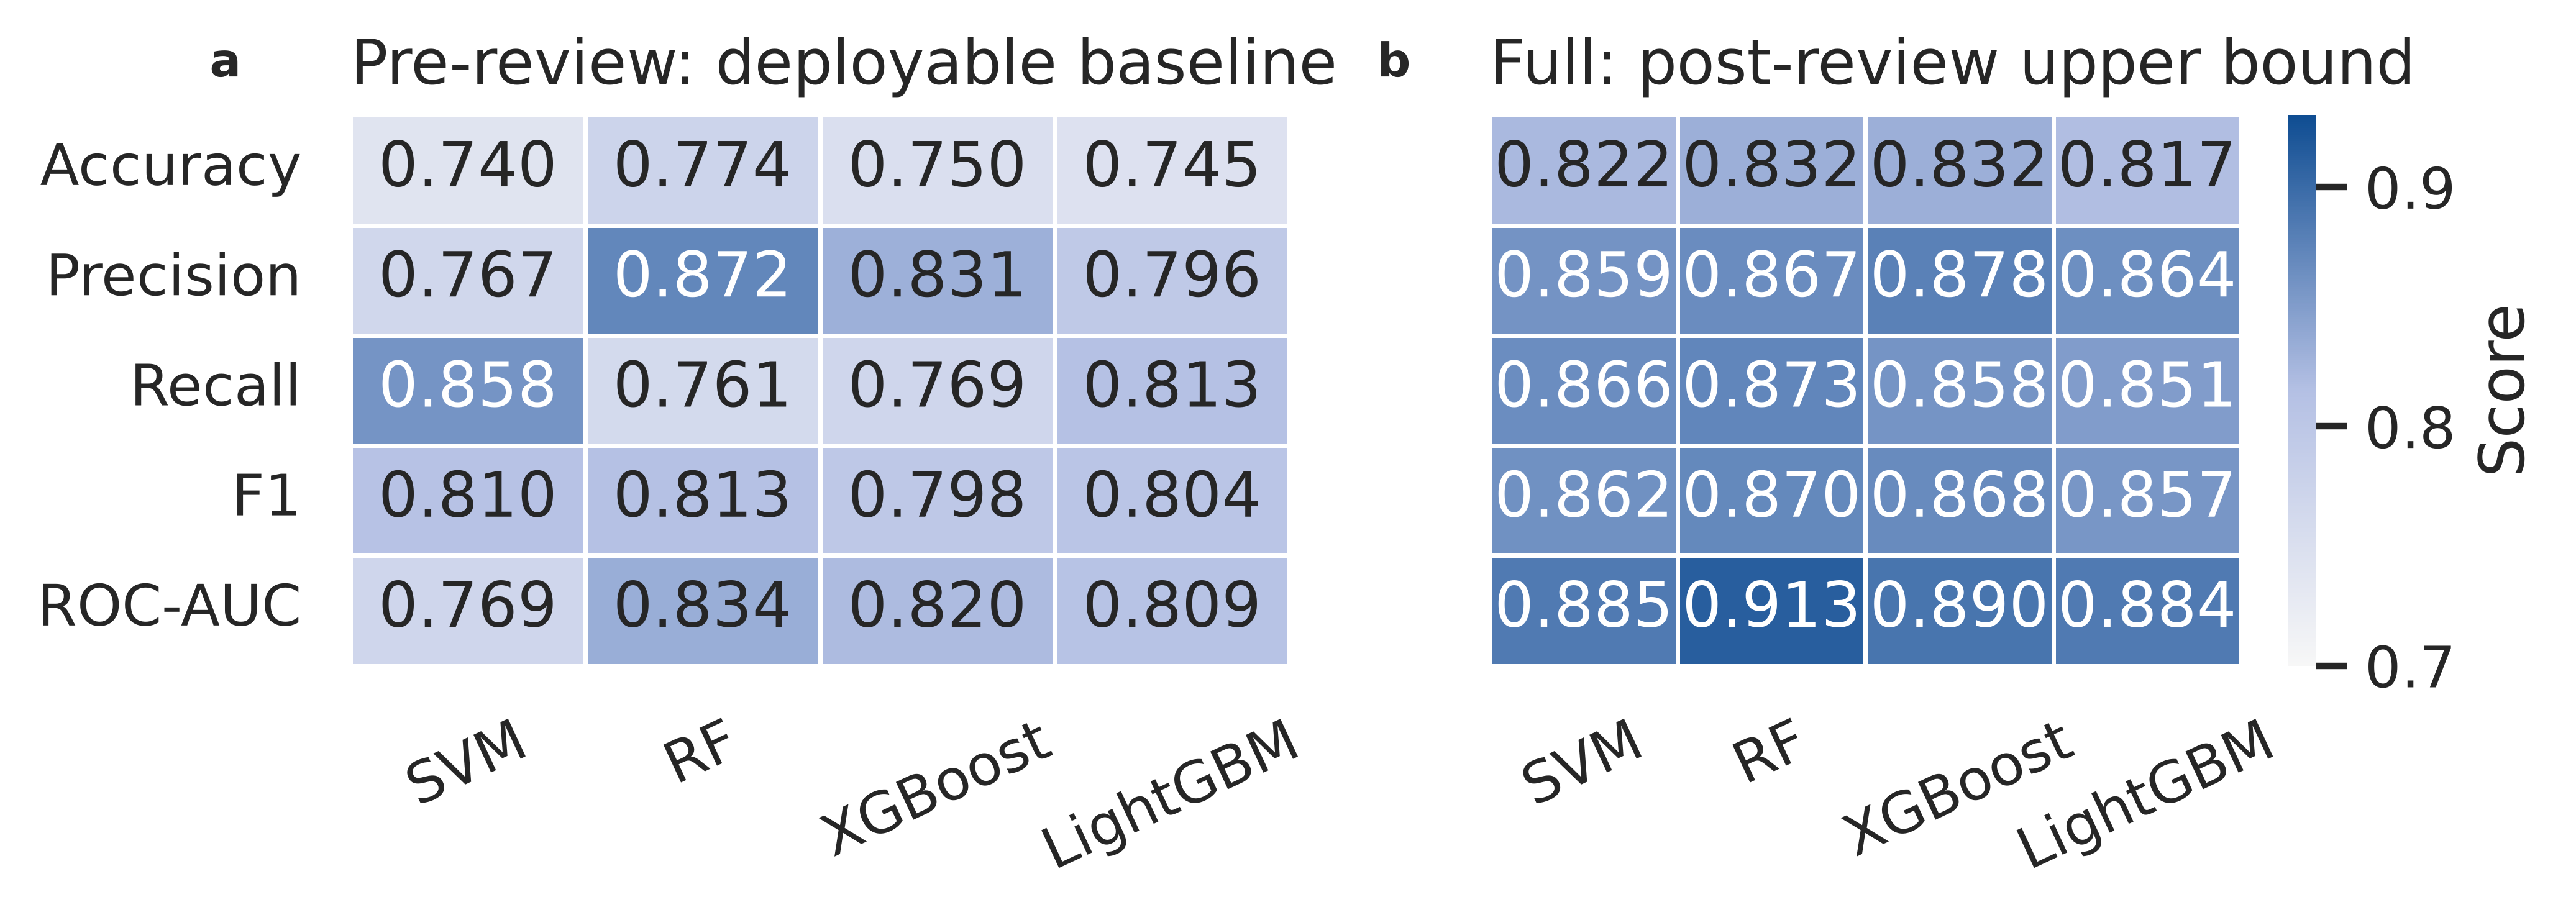
\includegraphics[width=0.95\textwidth]{model_performance_matrix.png}
\caption{\textbf{Merge Prediction 传统机器学习基线的测试集性能矩阵。} 热力图比较 SVM、RF、XGBoost 与 LightGBM 在两种特征设置下的表现：pre-review 设置仅使用 PR 提交时可获得的信息，full 设置额外纳入审查过程特征。各格给出在同一保留测试集（208 个 PR）上的 Accuracy、Precision、Recall、F1 与 ROC-AUC。}
\label{fig:matrix}
\end{figure}

\subsection*{3.2 标签泄漏消融}

为量化审查过程特征带来的时间泄漏影响，我们将每个模型从 pre-review 到 full 的 F1 变化连线对比（图~\ref{fig:ablation}）。所有模型加入 review 特征后均明显提升：SVM $0.810\rightarrow0.862$（$+0.052$）、RF $0.813\rightarrow0.870$（$+0.057$）、XGBoost $0.798\rightarrow0.868$（$+0.070$）、LightGBM $0.804\rightarrow0.857$（$+0.053$）。其中 XGBoost 增幅最大，说明 boosting 模型能更充分利用审查次数、审查者数量与评论密度等后验信号。这一结果给出一条重要的方法论边界：若仅报告 full 性能，会高估模型在真实前置预测中的表现。因此对后续实验三、四、七而言，应以 pre-review 结果作为可部署基线，而将 full 结果作为含时间泄漏的上界参考。

\begin{figure}[H]
\centering
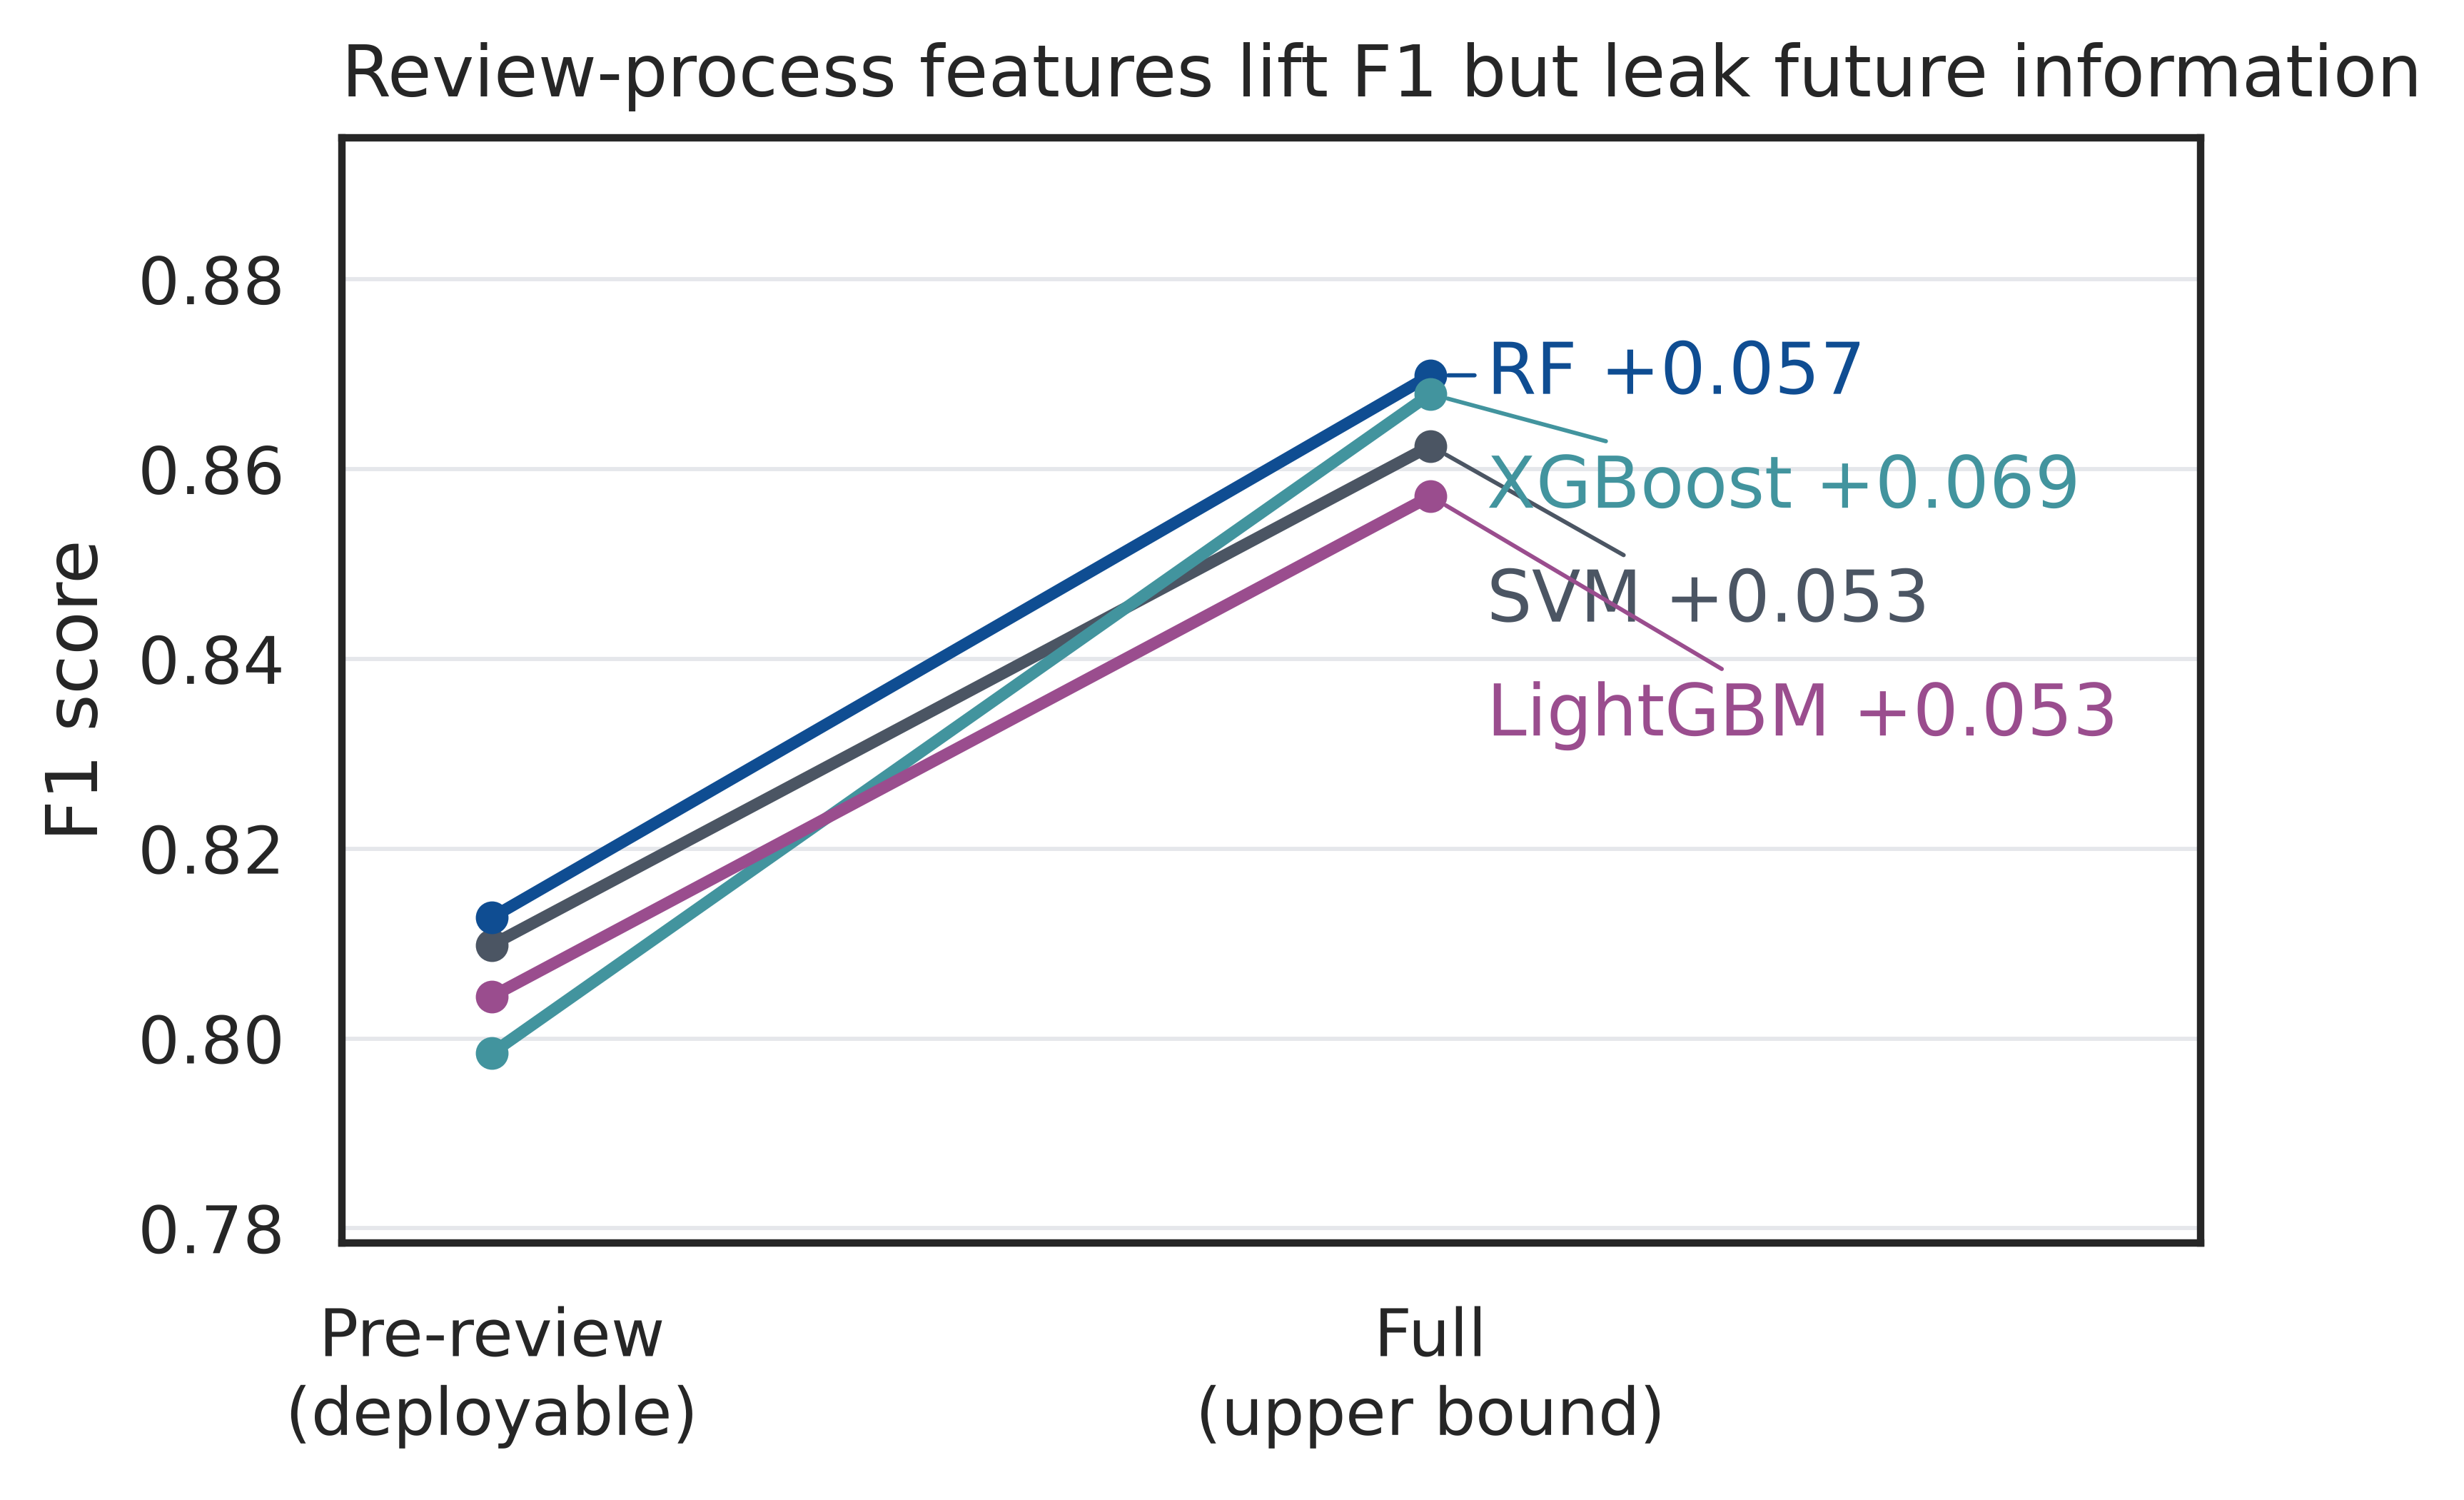
\includegraphics[width=0.7\textwidth]{label_leakage_ablation.png}
\caption{\textbf{可部署设置与含审查过程设置之间的标签泄漏消融。} 连线表示每个模型的 F1 从 pre-review 特征到 full 特征的变化，右侧标注审查过程特征引入的 F1 增量。所有模型的增量集中在 $+0.05\sim+0.07$，其中 XGBoost 最大。}
\label{fig:ablation}
\end{figure}

\subsection*{3.3 判别能力与错误结构}

我们进一步用 ROC 曲线刻画阈值无关的排序能力（图~\ref{fig:roc-pre}、图~\ref{fig:roc-full}），并用混淆矩阵分析具体误判类型（图~\ref{fig:cm-pre}、图~\ref{fig:cm-full}）。在 pre-review 设置下（图~\ref{fig:roc-pre}），RF 的 ROC-AUC 最高（0.834），XGBoost、LightGBM、SVM 依次为 0.820、0.809、0.769，排序与 F1 一致，说明 RF 在不同阈值下均保持更稳定的区分能力；但 pre-review AUC 尚未达到 full 水平，反映仅凭提交时特征难以完全排序部分边界样本——这与代码审查任务的本质一致，PR 是否合并不仅取决于 diff，还受维护者反馈、项目计划与后续修改等过程因素影响。加入审查过程特征后（图~\ref{fig:roc-full}），所有模型 AUC 均升至 0.884 以上，RF 达 0.913（较 pre-review 提升约 0.079），但该曲线应解读为含未来信息的预测上界，而非实验七插件在 PR 提交时的目标性能。

\begin{figure}[H]
\centering
\begin{subfigure}{0.49\textwidth}
  \centering
  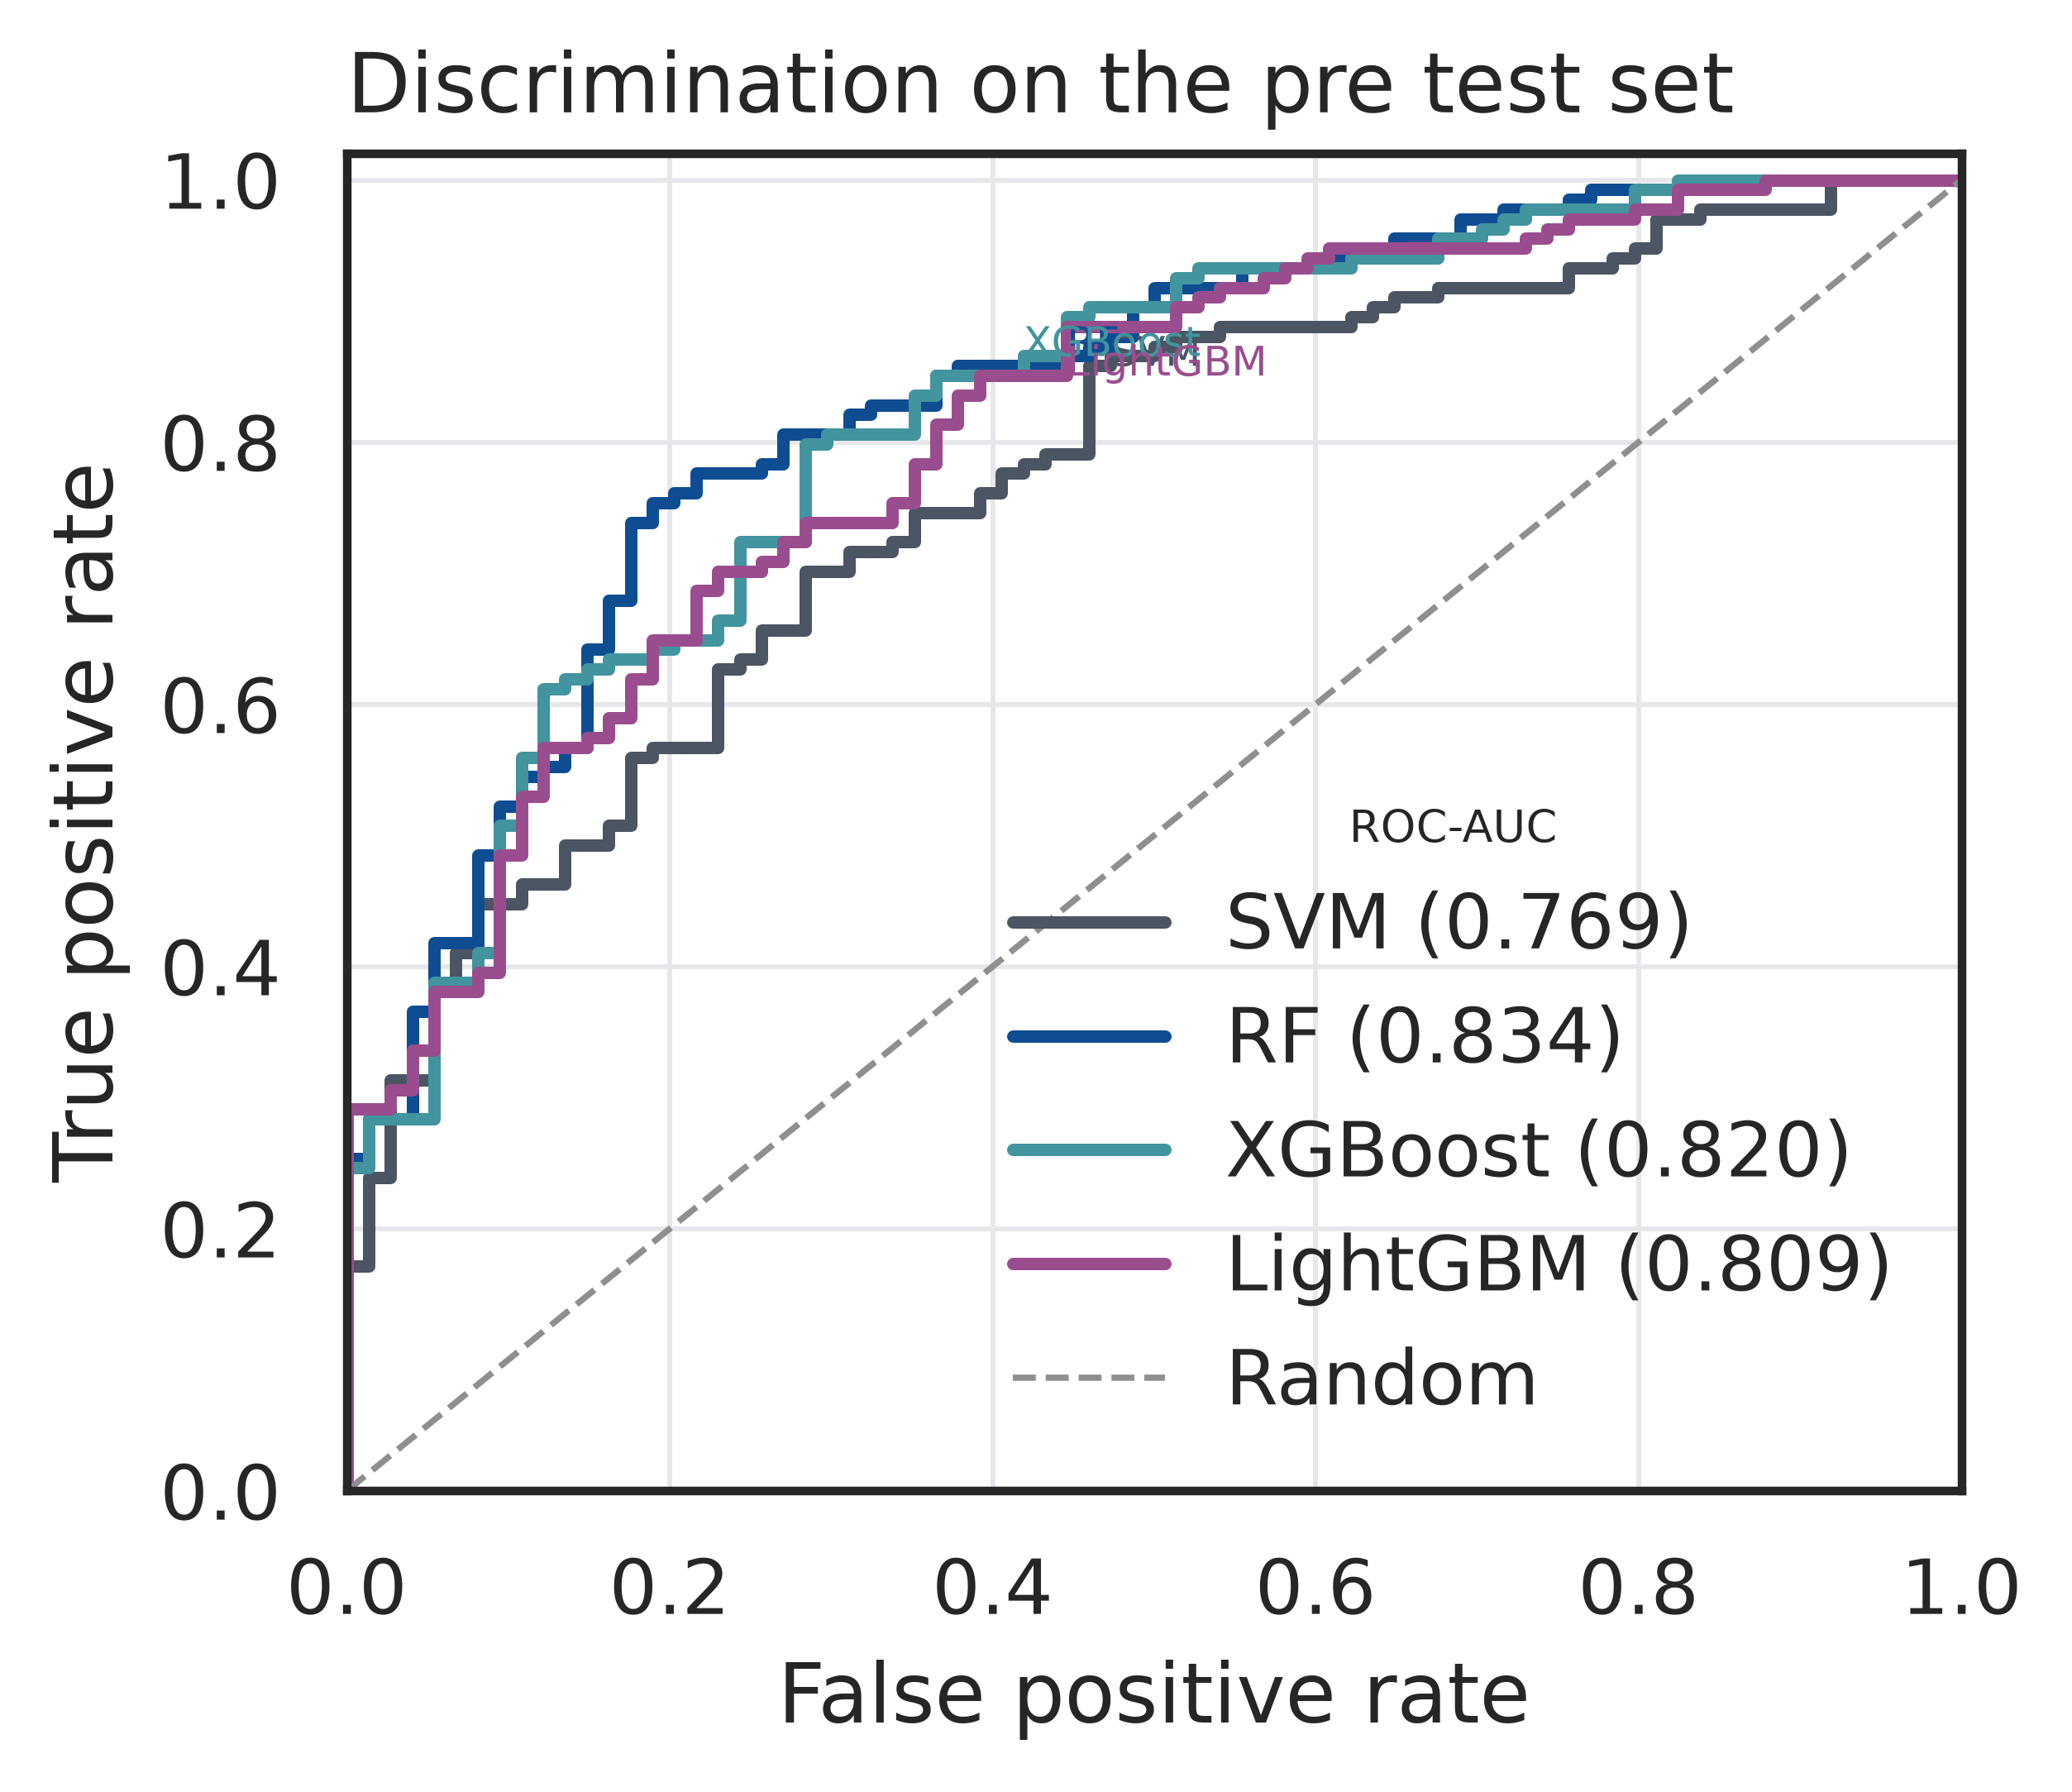
\includegraphics[width=\textwidth]{roc_curves_pre.png}
  \caption{Pre-review 设置}
  \label{fig:roc-pre}
\end{subfigure}
\hfill
\begin{subfigure}{0.49\textwidth}
  \centering
  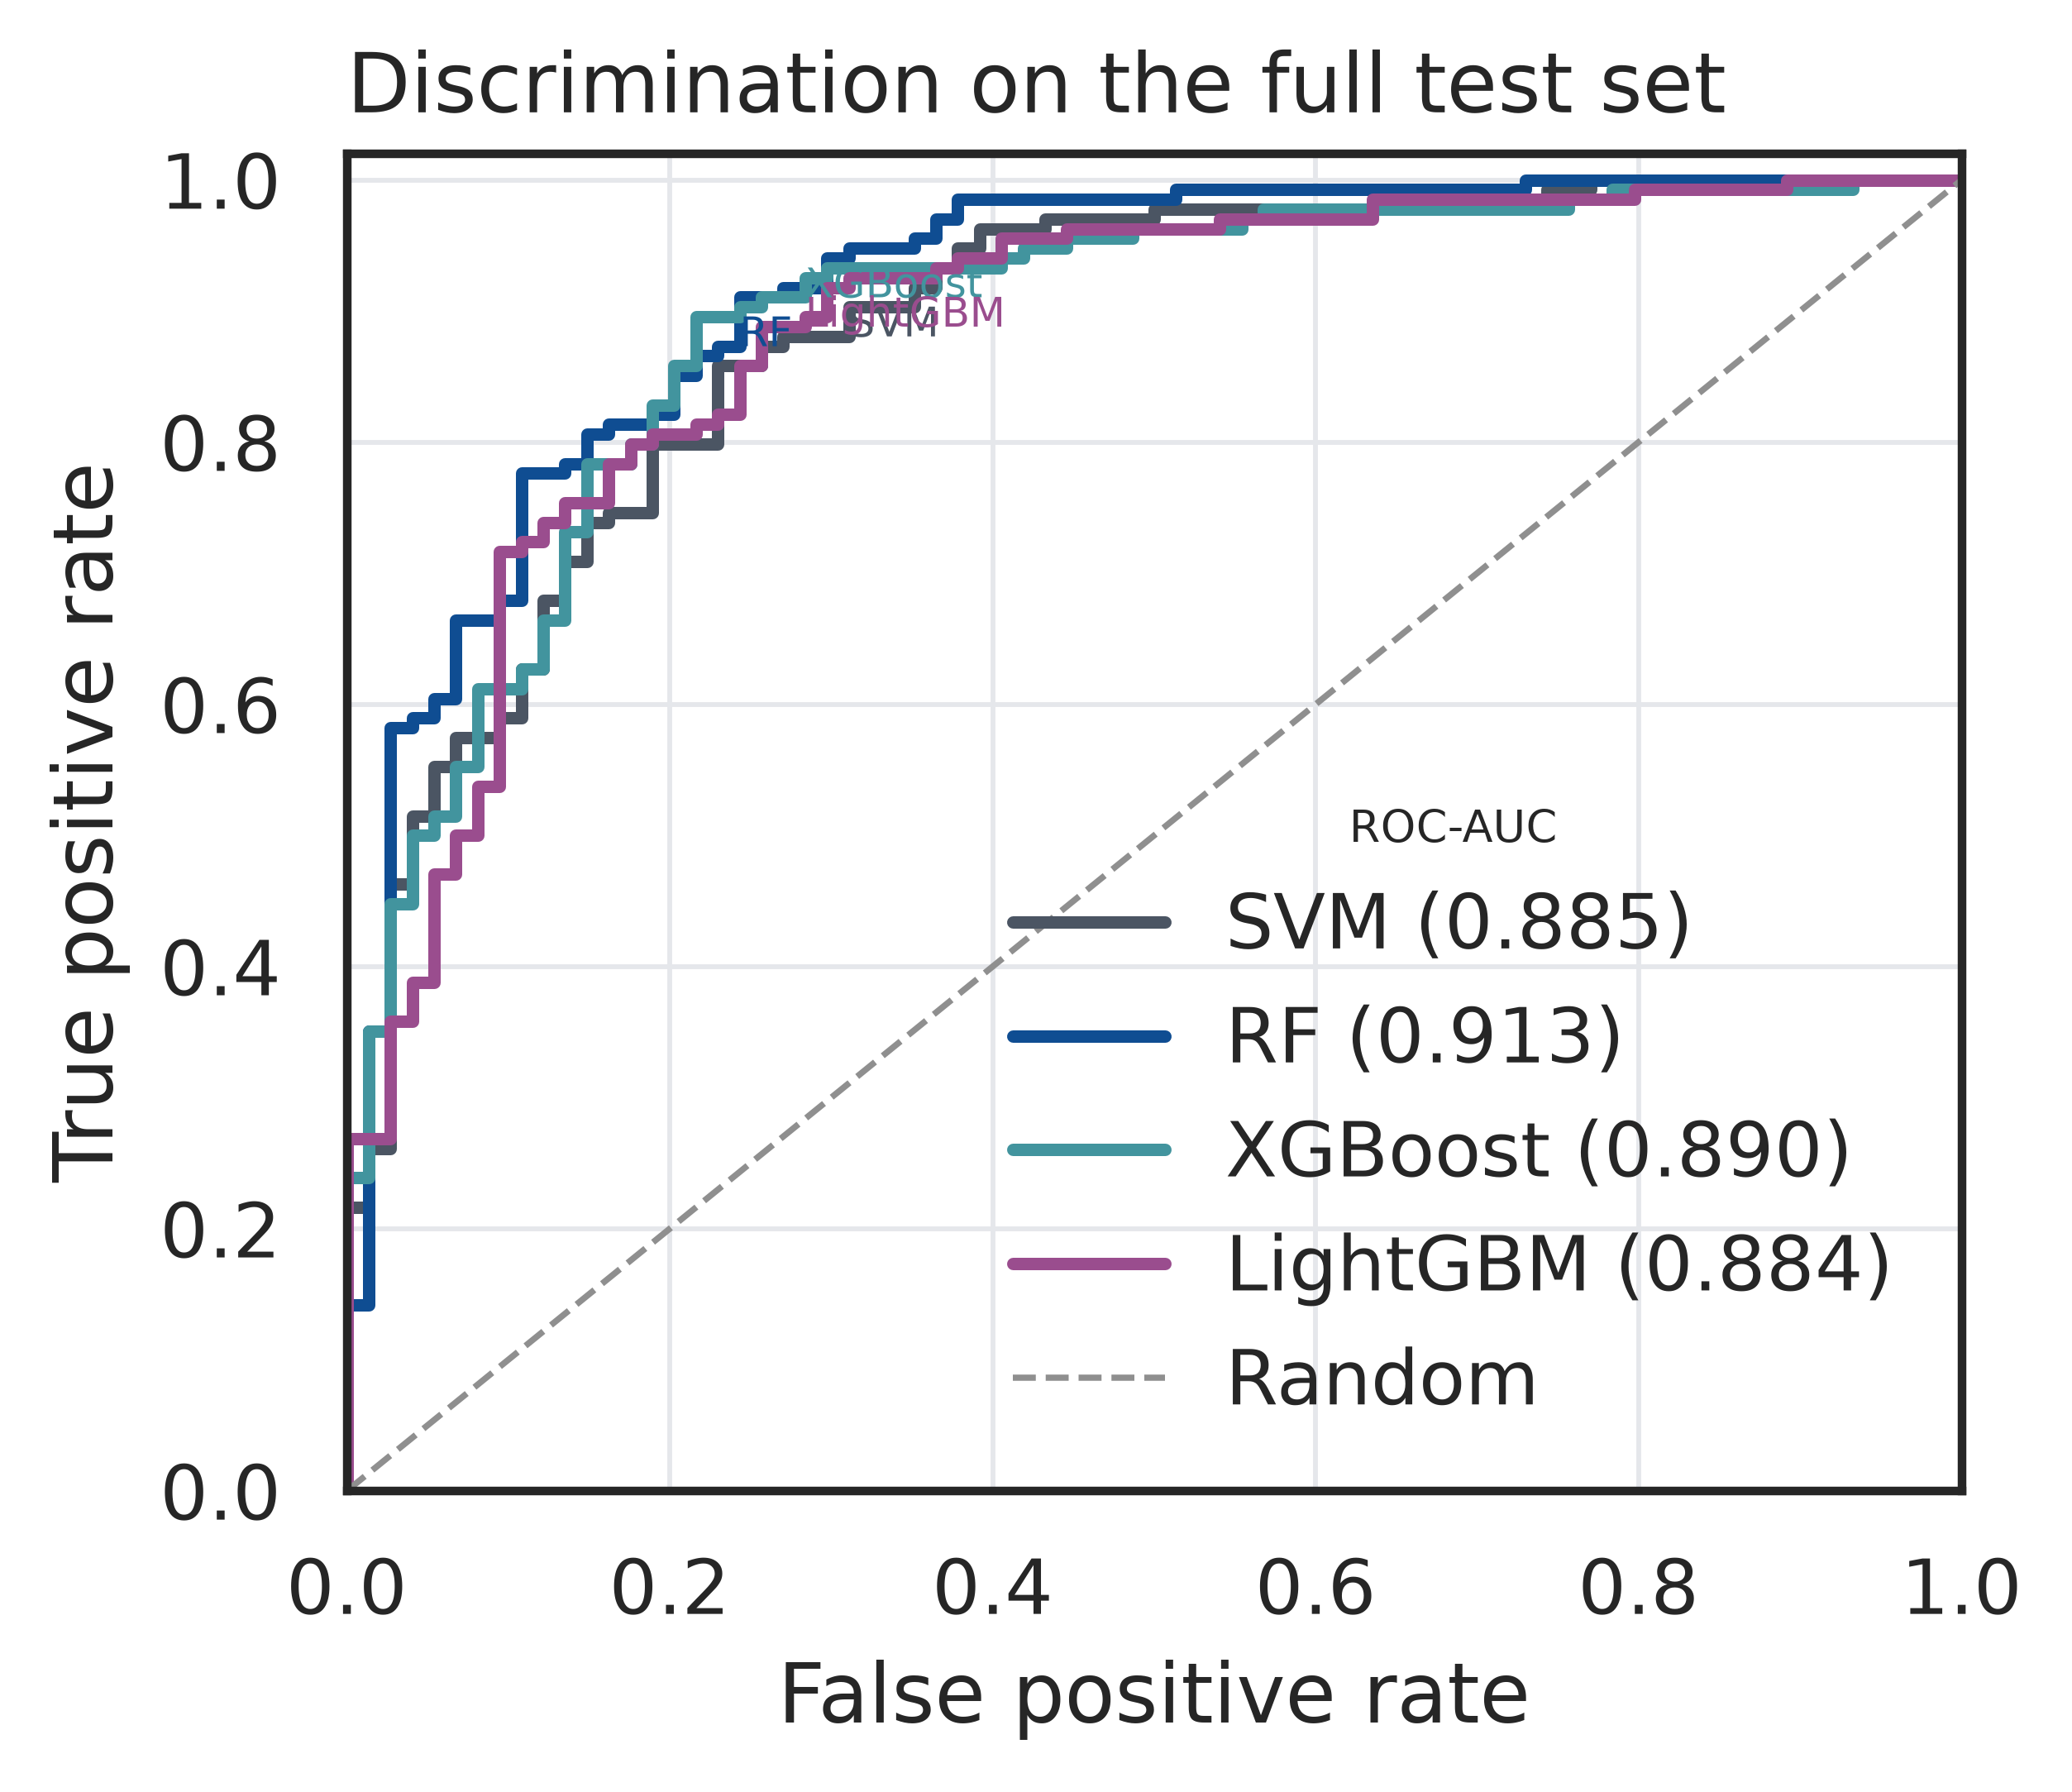
\includegraphics[width=\textwidth]{roc_curves_full.png}
  \caption{Full 设置}
  \label{fig:roc-full}
\end{subfigure}
\caption{\textbf{两种特征设置下 Merge Prediction 模型的 ROC 曲线。} 曲线给出保留测试集上真正例率对假正例率的关系。(a) pre-review 仅用可部署特征，RF 的 AUC 最高（0.834）；(b) full 纳入审查过程特征，代表上界分析而非可部署协议，RF 的 AUC 升至 0.913。}
\label{fig:roc}
\end{figure}

混淆矩阵揭示了误判的具体结构。在 pre-review 设置下（图~\ref{fig:cm-pre}），SVM 正确识别 115 个 merged PR 但将 35 个 non-merged PR 误判为 merged，呈明显的合并倾向（与其高 recall、低 precision 一致）；RF 将 non-merged 的误判降至 15 个，是对负类最谨慎的模型，但同时漏掉 32 个实际 merged PR。XGBoost（21 个假正例 / 31 个假负例）与 LightGBM（28 / 25）介于二者之间。据此可得部署取舍结论：若目标是降低“把不可合并 PR 误判为可合并”的风险，RF 更合适；若目标是尽可能召回可合并 PR，SVM 或 LightGBM 可作补充。加入审查过程特征后（图~\ref{fig:cm-full}），各模型误判整体下降——RF 的假负例从 32 降至 17、假正例仅从 15 微升至 18，SVM 假正例从 35 降至 19，LightGBM 假正例从 28 降至 18——说明 review 特征使模型更易同时识别两类样本，但该改进仍来自后验信息。

\begin{figure}[H]
\centering
\begin{subfigure}{0.49\textwidth}
  \centering
  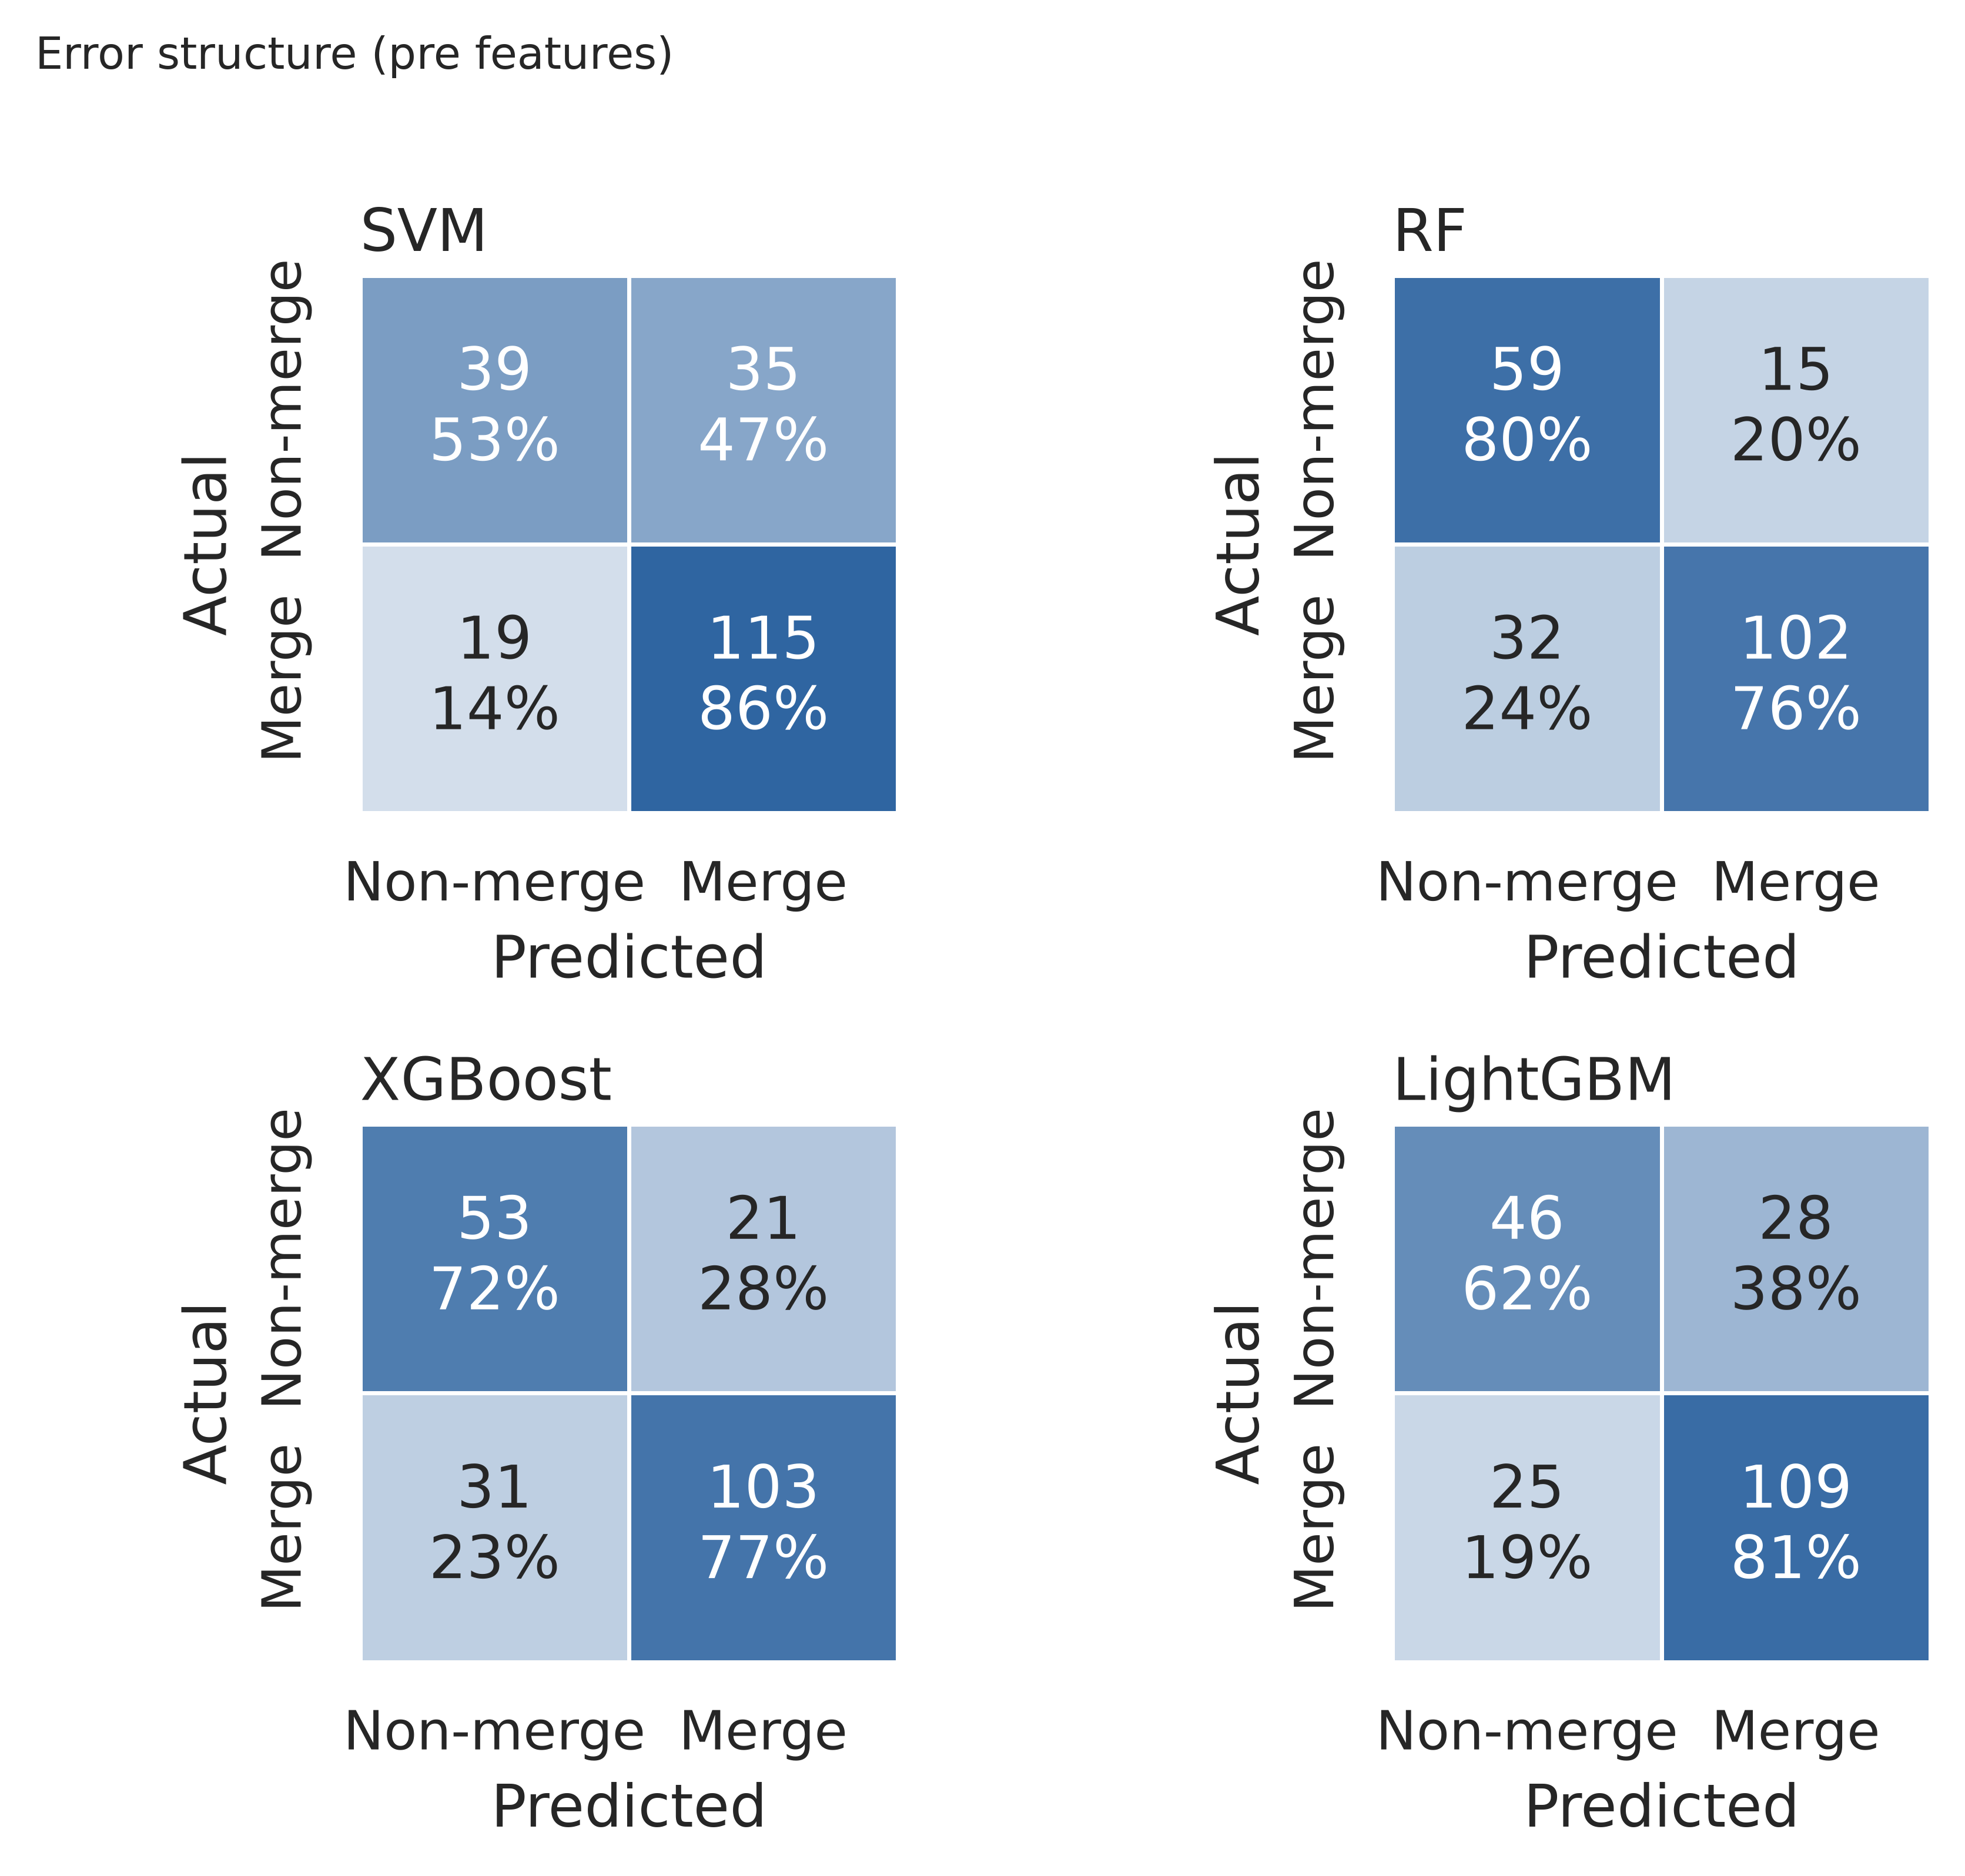
\includegraphics[width=\textwidth]{confusion_matrices_pre.png}
  \caption{Pre-review 设置}
  \label{fig:cm-pre}
\end{subfigure}
\hfill
\begin{subfigure}{0.49\textwidth}
  \centering
  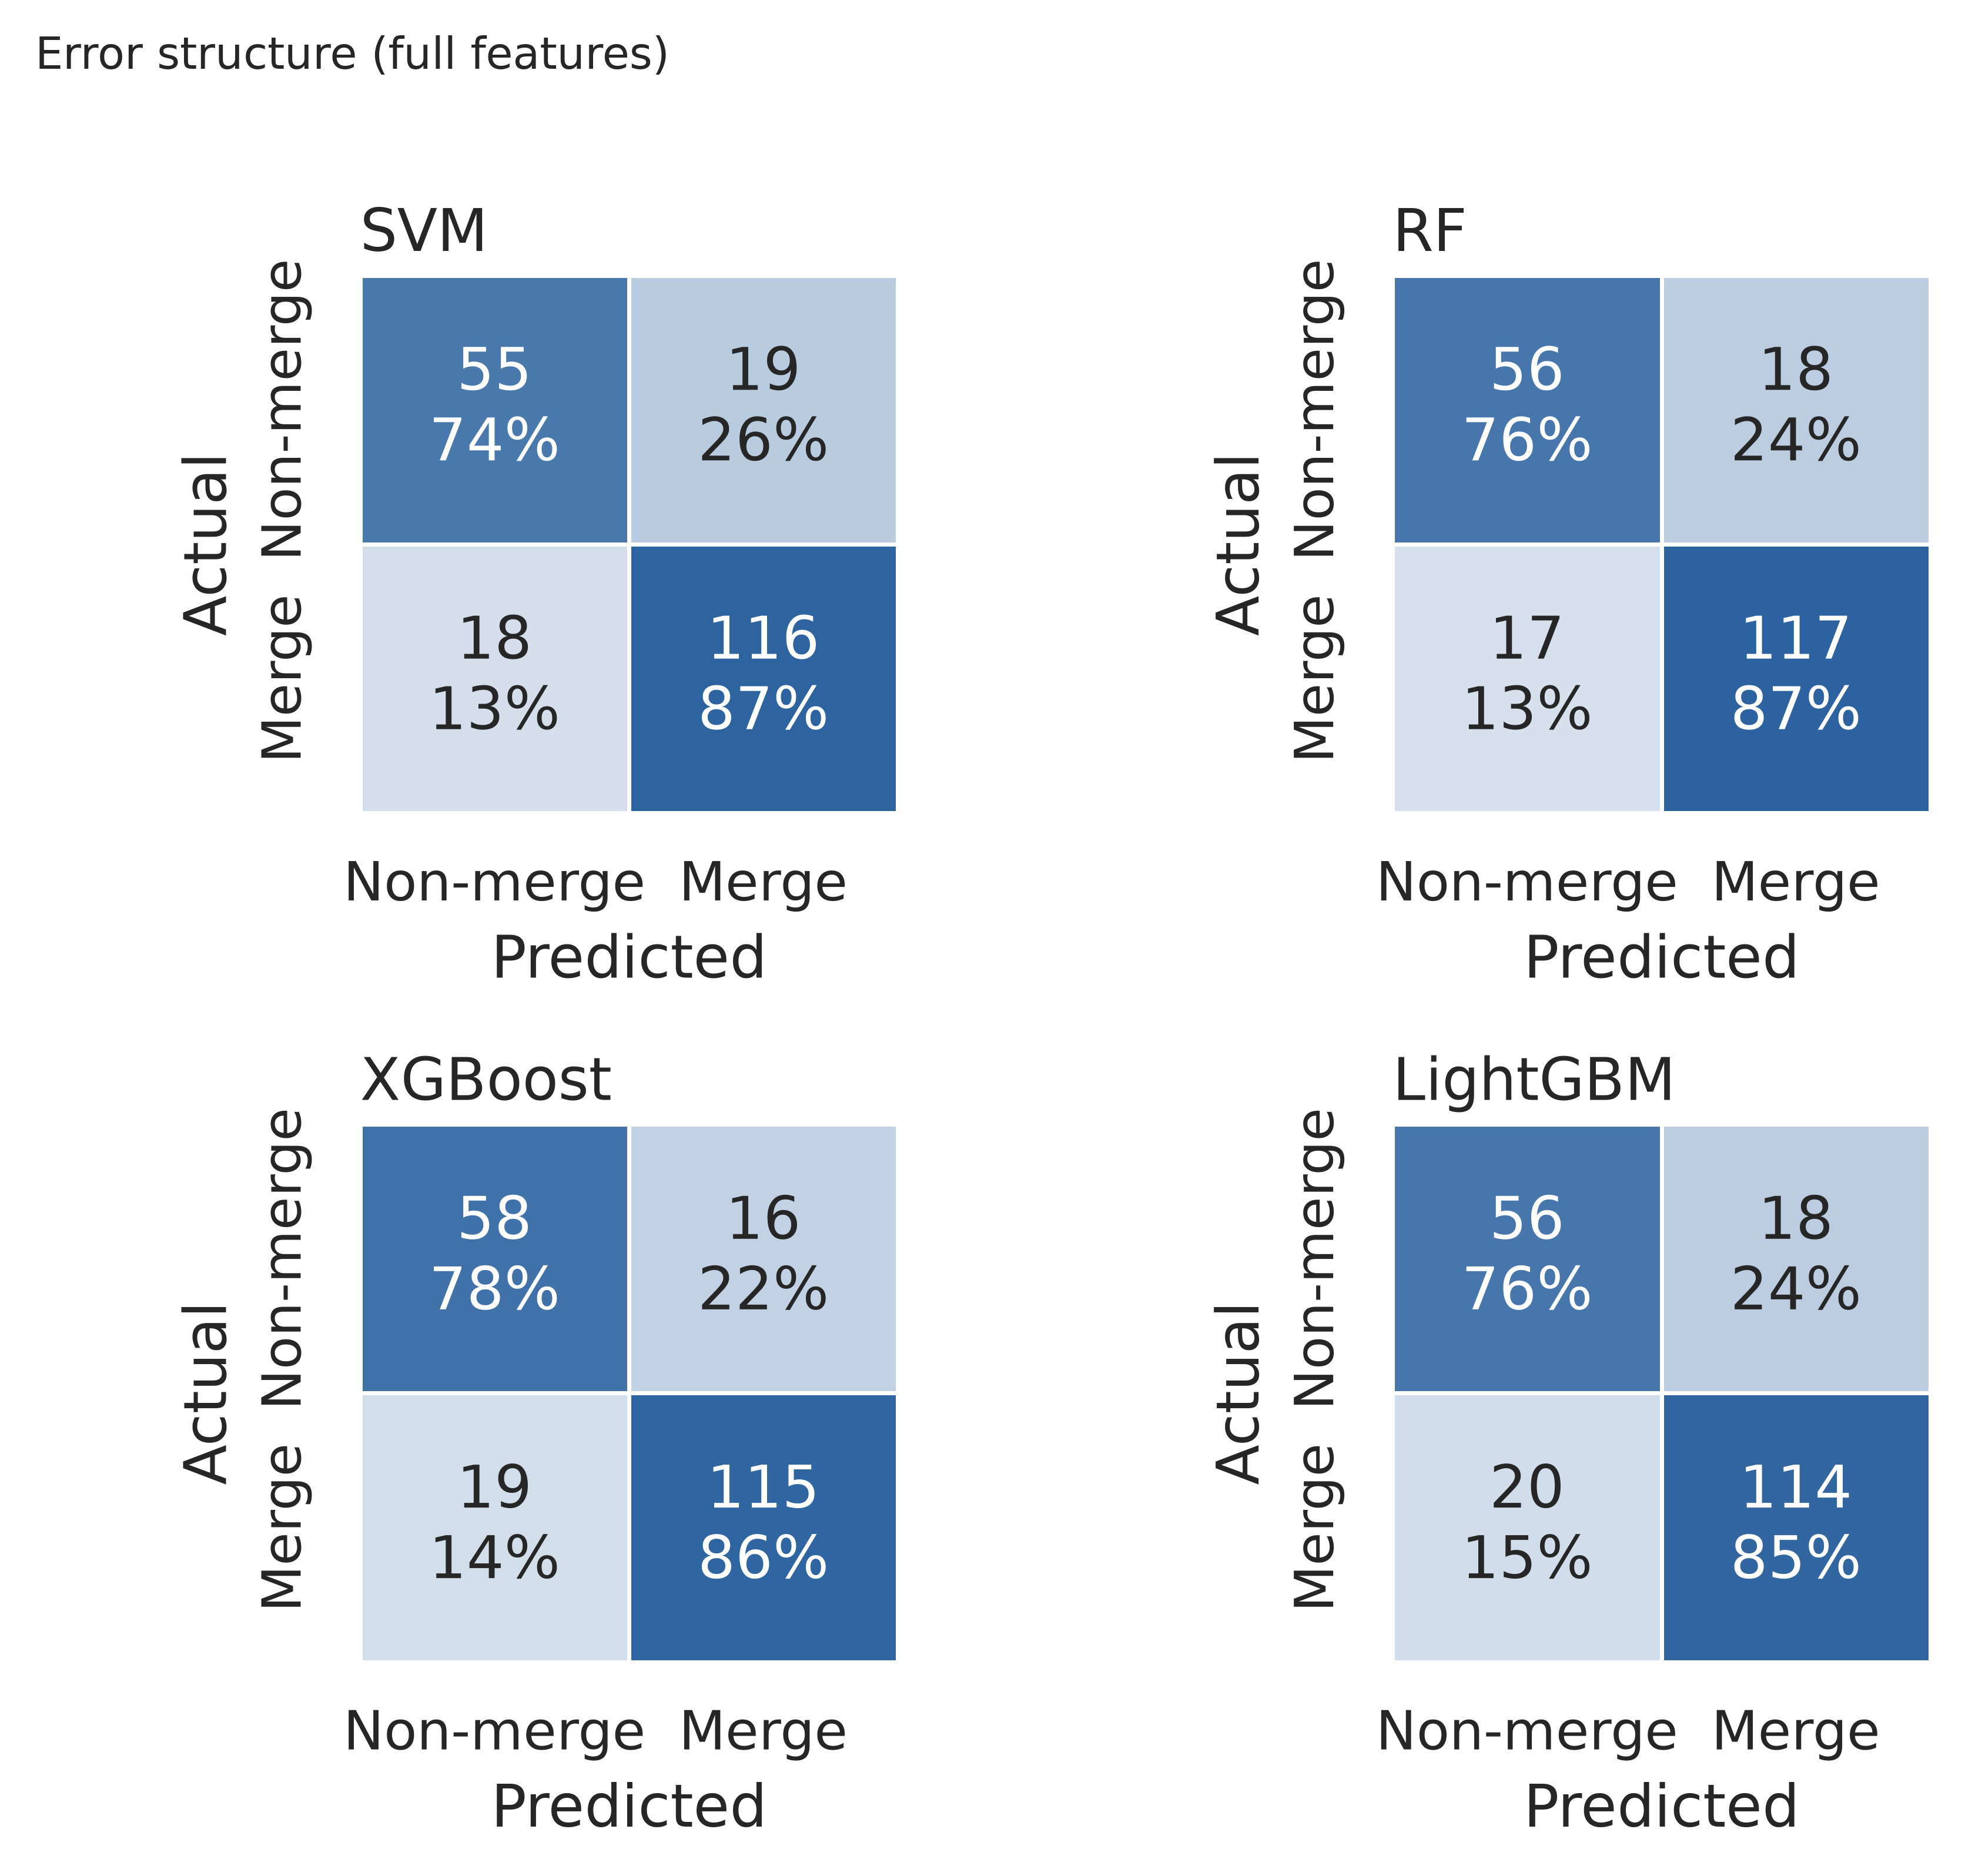
\includegraphics[width=\textwidth]{confusion_matrices_full.png}
  \caption{Full 设置}
  \label{fig:cm-full}
\end{subfigure}
\caption{\textbf{两种特征设置下各模型在保留测试集上的混淆矩阵。} 每格给出 PR 数量与按行归一化的比例（实际 non-merged 与 merged 两类）。相比 pre-review，full 设置对多数分类器同时减少了假正例与假负例。}
\label{fig:cm}
\end{figure}

\subsection*{3.4 特征重要性（可解释性分析）}

我们读取 RF 的 Gini 重要性以回答“哪类特征贡献最大”。在无泄漏的 pre-review 设置下（图~\ref{fig:fi-pre}），文本特征构成最主要信号：最重要的单个特征为 \texttt{tfidf\_github}（0.0595），其后依次为 \texttt{tfidf\_py}（0.0414）、\texttt{avg\_commit\_msg\_len}（0.0310）、\texttt{tfidf\_pull}（0.0264）、\texttt{title\_len}（0.0246）与 \texttt{body\_len}（0.0228）；改动量特征 \texttt{deletions}、\texttt{churn\_ratio}、\texttt{additions} 及 AST 结构特征 \texttt{ast\_avg\_branching}、\texttt{ast\_max\_depth} 提供辅助信号，而 CFG 特征在家族汇总中贡献较弱。值得注意的是 \texttt{tfidf\_github} 高居榜首：经查约 50\% 的人类 PR 正文含 github.com 链接（引用相关 issue/PR），这类 PR 合并率达 81.5\%，远高于不含链接者的约 49\%——这是一个合理的\textbf{提交时质量信号}（引用了上下文的 PR 通常更规范、更易合并），而非泄漏。据此得出结论：在真实部署设置中，文本上下文与改动规模是 Merge Prediction 的主要人工信号，AST 结构提供次级解释力，CFG 贡献较小。

\begin{figure}[H]
\centering
\begin{subfigure}{0.49\textwidth}
  \centering
  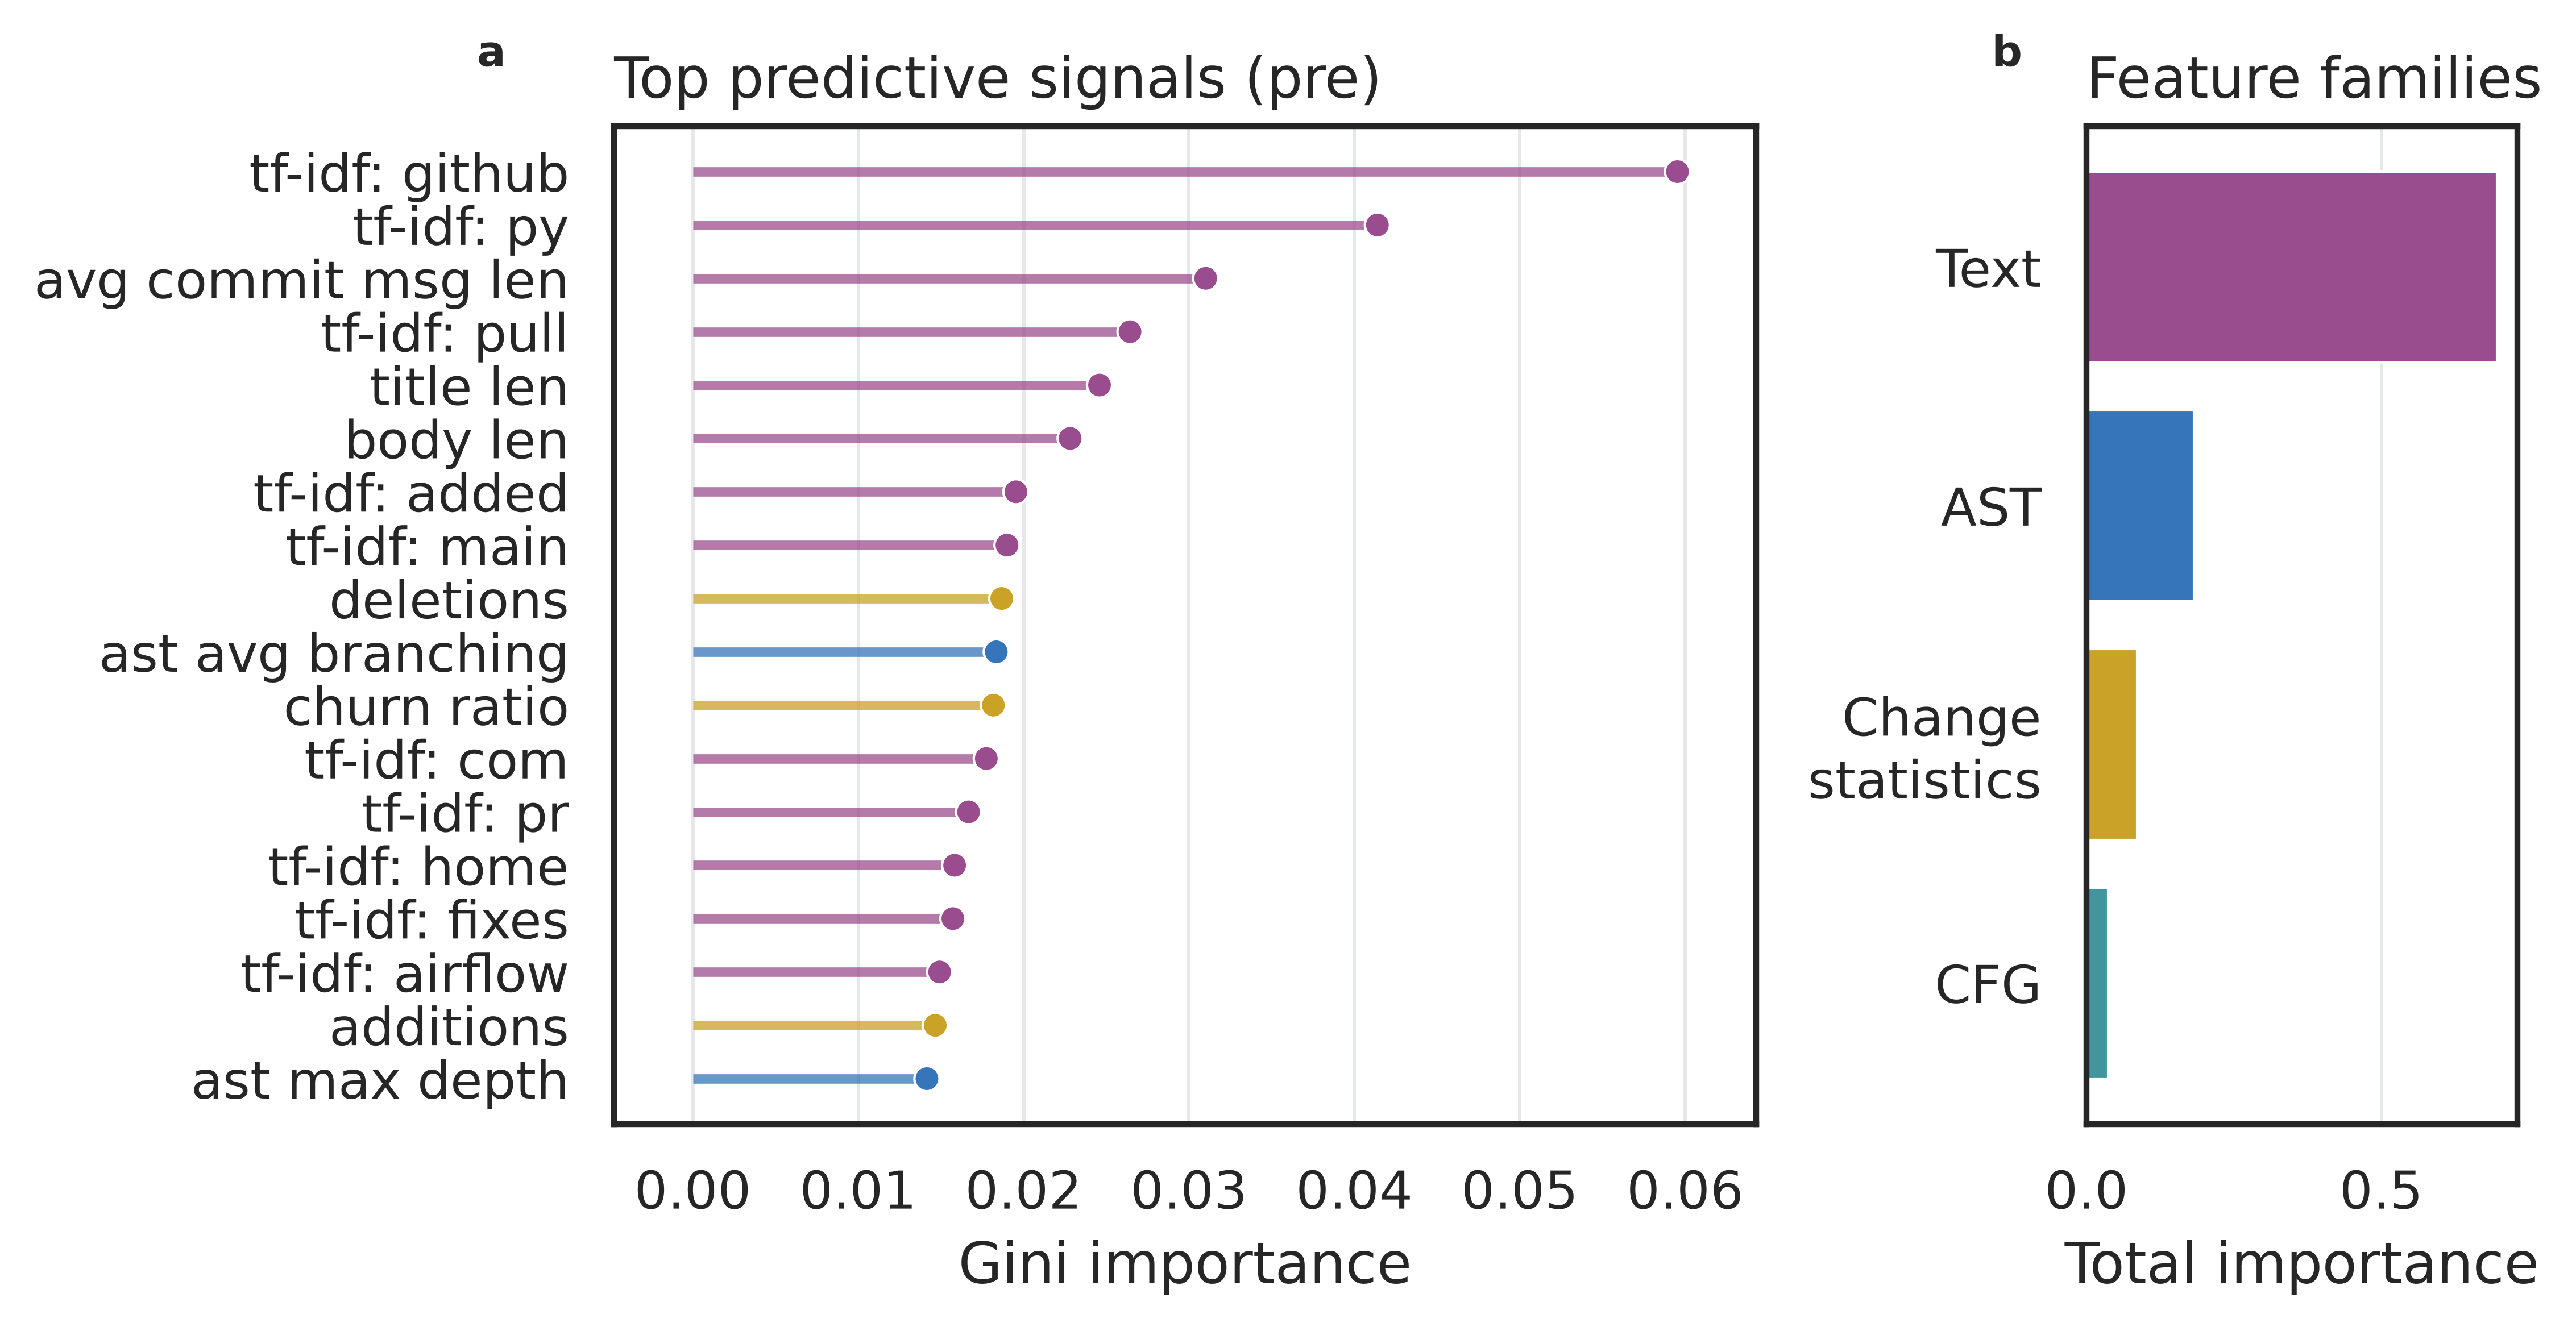
\includegraphics[width=\textwidth]{feature_importance_rf_pre.png}
  \caption{Pre-review 设置}
  \label{fig:fi-pre}
\end{subfigure}
\hfill
\begin{subfigure}{0.49\textwidth}
  \centering
  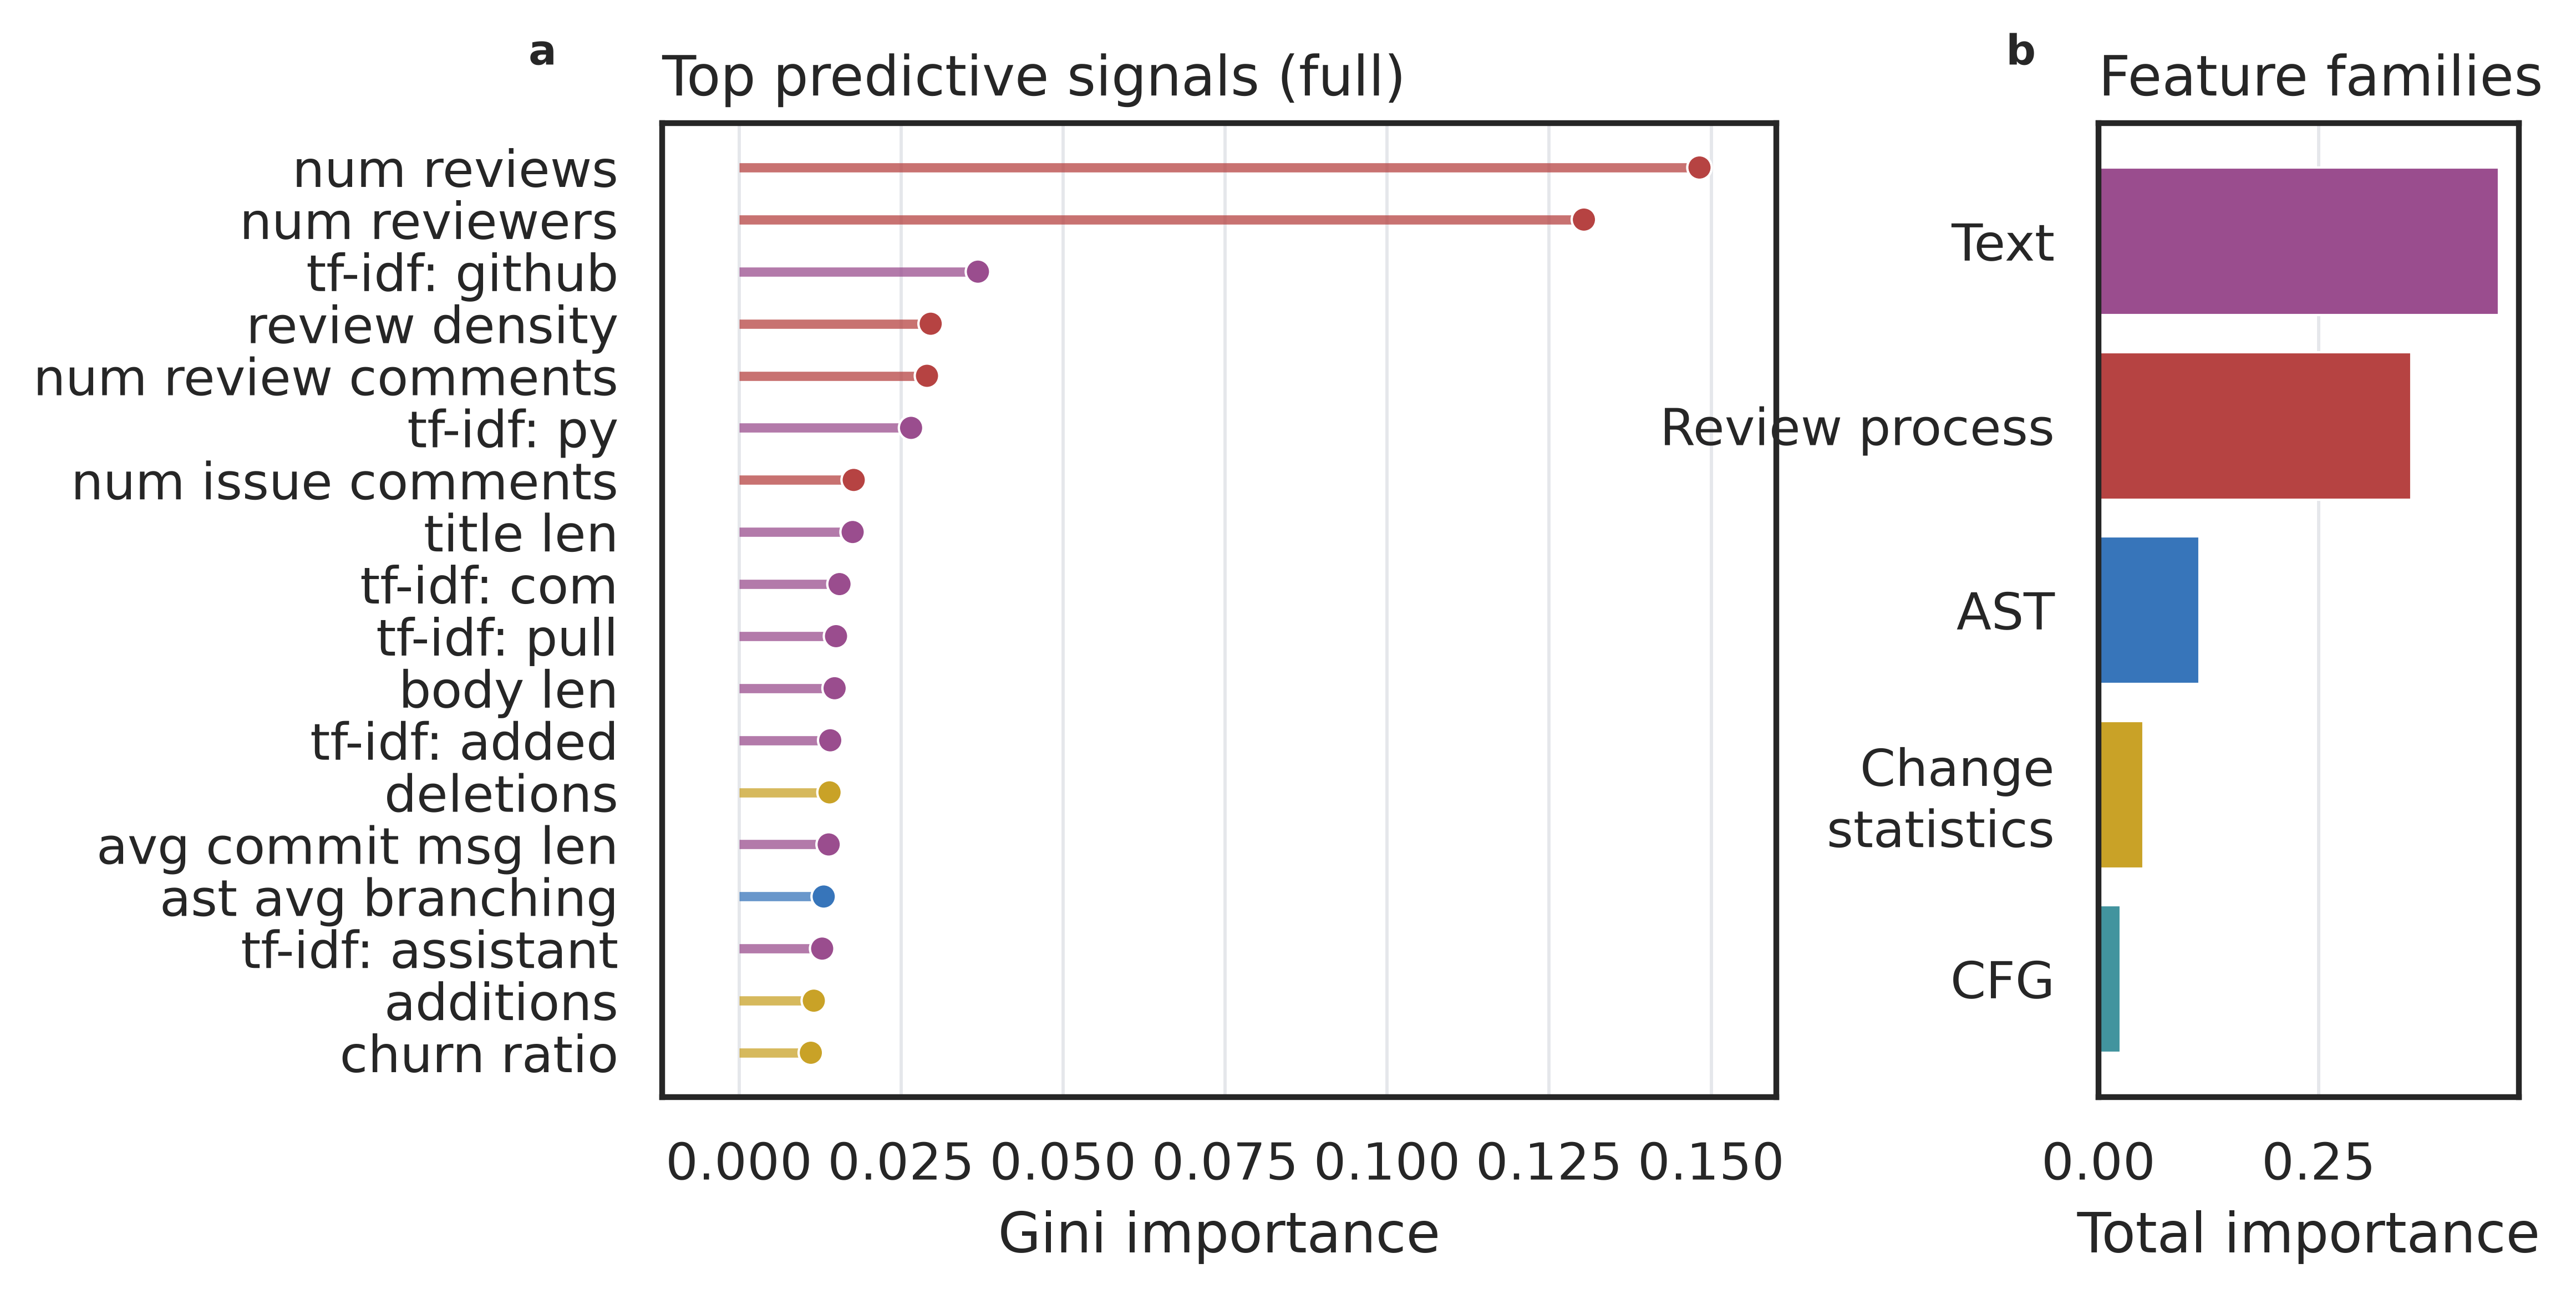
\includegraphics[width=\textwidth]{feature_importance_rf_full.png}
  \caption{Full 设置}
  \label{fig:fi-full}
\end{subfigure}
\caption{\textbf{Random Forest 的特征重要性。} 颜色区分文本、AST、CFG、改动统计与审查过程特征。(a) 可部署 RF 中文本上下文与改动规模主导；(b) full RF 中 \texttt{num\_reviews} 与 \texttt{num\_reviewers} 等审查过程特征主导，直接解释了上界模型的性能来源。}
\label{fig:fi}
\end{figure}

在 full 设置下（图~\ref{fig:fi-full}），最重要的两个特征变为 \texttt{num\_reviews}（0.1482）与 \texttt{num\_reviewers}（0.1304），二者合计约占 28\%，显著高于所有 pre-review 特征；\texttt{review\_density}（0.0296）、\texttt{num\_review\_comments}（0.0290）、\texttt{num\_issue\_comments}（0.0177）亦进入前列，而 \texttt{tfidf\_github} 虽仍保留一定重要性（0.0369），相对地位已被审查过程变量超过。这直接解释了 3.2 节 full 设置的性能提升来源：模型并非仅通过更好地理解 diff 而提升，而是利用了 PR 在审查过程中产生的交互强度。审查次数、审查者数量与评论密度很可能与维护者关注度、讨论充分性及最终合并决策高度相关，但它们在 PR 创建时不可获得，因此验证了标签泄漏消融的必要性。

\subsection*{3.5 跨仓库泛化}

为检验实验一 EDA 提示的分布偏移，我们按仓库分解 F1（图~\ref{fig:repo-pre}、图~\ref{fig:repo-full}）。在 pre-review 设置下（图~\ref{fig:repo-pre}），模型性能受项目合并率与审查文化显著影响：合并率最高的 \texttt{home-assistant/core}（92.0\%）各模型 F1 均达 0.963 以上（RF 0.975），\texttt{apache/airflow}（80.7\%）稳定在 0.818--0.848；而合并率最低、类别最均衡的 \texttt{django/django}（46.7\%）pre-review RF F1 仅 0.500，\texttt{pandas-dev/pandas}（52.6\%）RF F1 为 0.720。这说明整体平均指标会掩盖仓库级分布偏移，报告传统 ML 基线时必须同时展示分仓库性能。在 full 设置下（图~\ref{fig:repo-full}），困难仓库提升最明显：\texttt{django/django} 的 RF F1 从 0.500 跃升至 0.800、XGBoost 从 0.541 升至 0.808；而高合并率的 \texttt{home-assistant/core} 几乎不再提升（RF 0.975 微降至 0.963）。据此得出结论：Merge Prediction 难度具有强仓库依赖性，审查过程特征对低合并率、结局更不确定的仓库价值最大，这进一步指明仓库级上下文与审查过程信息是后续实验的重要改进方向。

\begin{figure}[H]
\centering
\begin{subfigure}{0.49\textwidth}
  \centering
  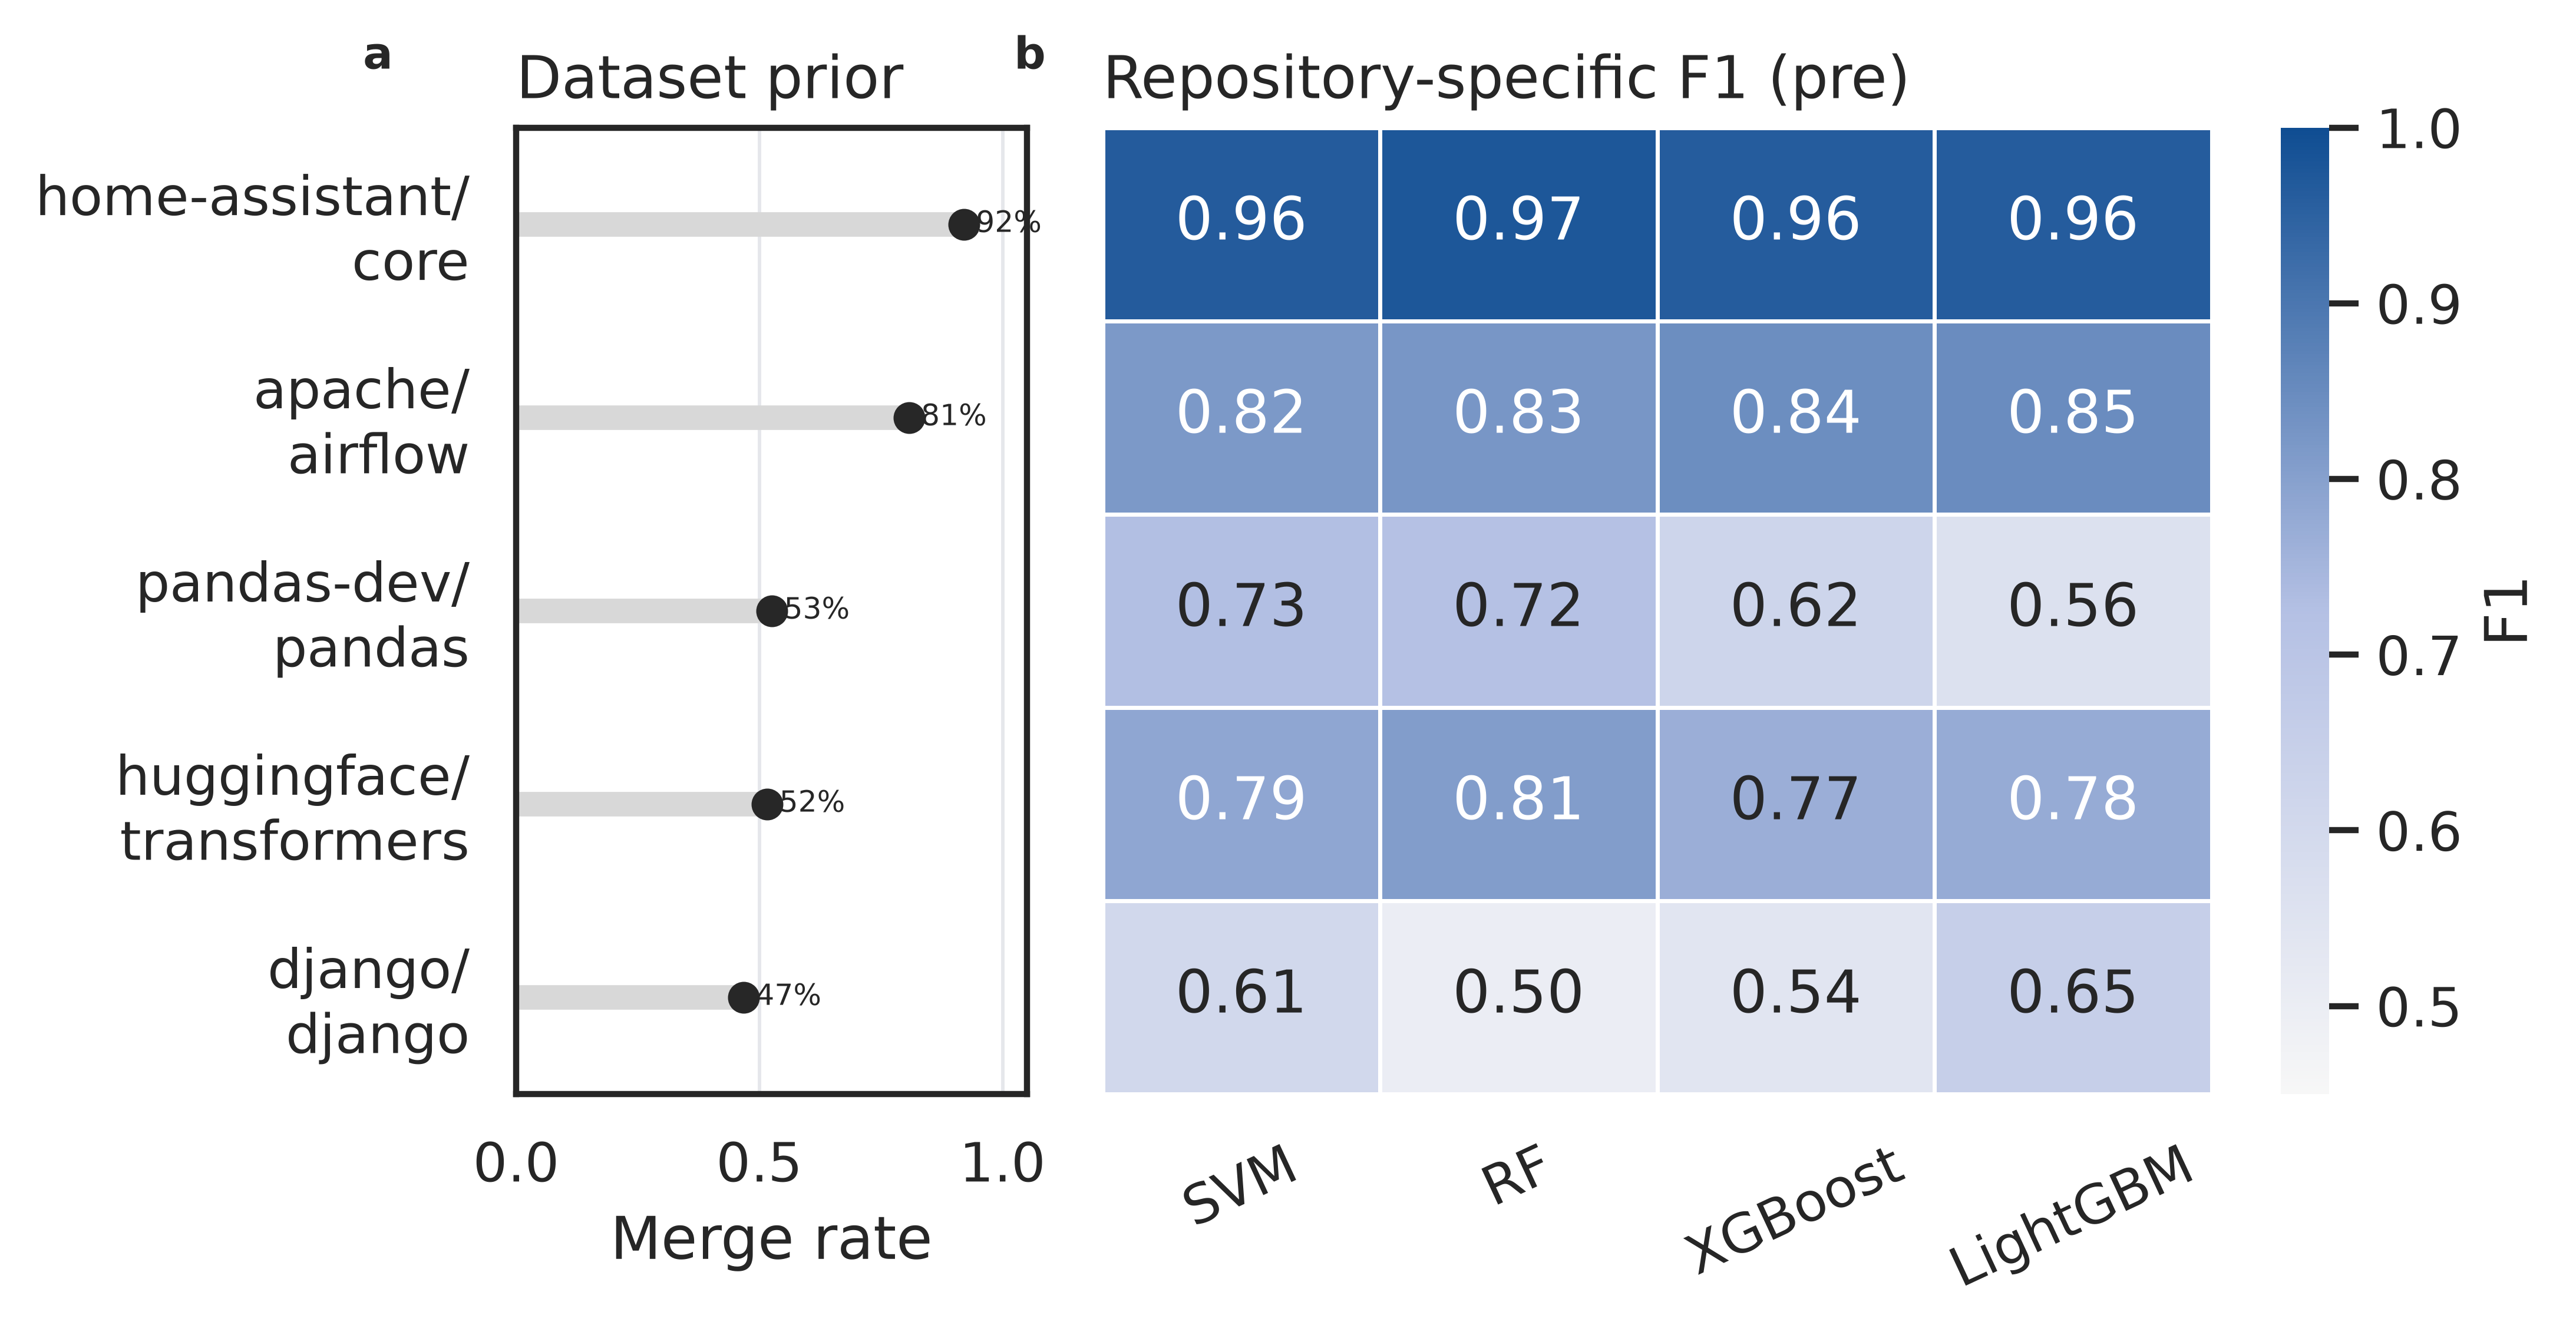
\includegraphics[width=\textwidth]{cross_repo_performance_pre.png}
  \caption{Pre-review 设置}
  \label{fig:repo-pre}
\end{subfigure}
\hfill
\begin{subfigure}{0.49\textwidth}
  \centering
  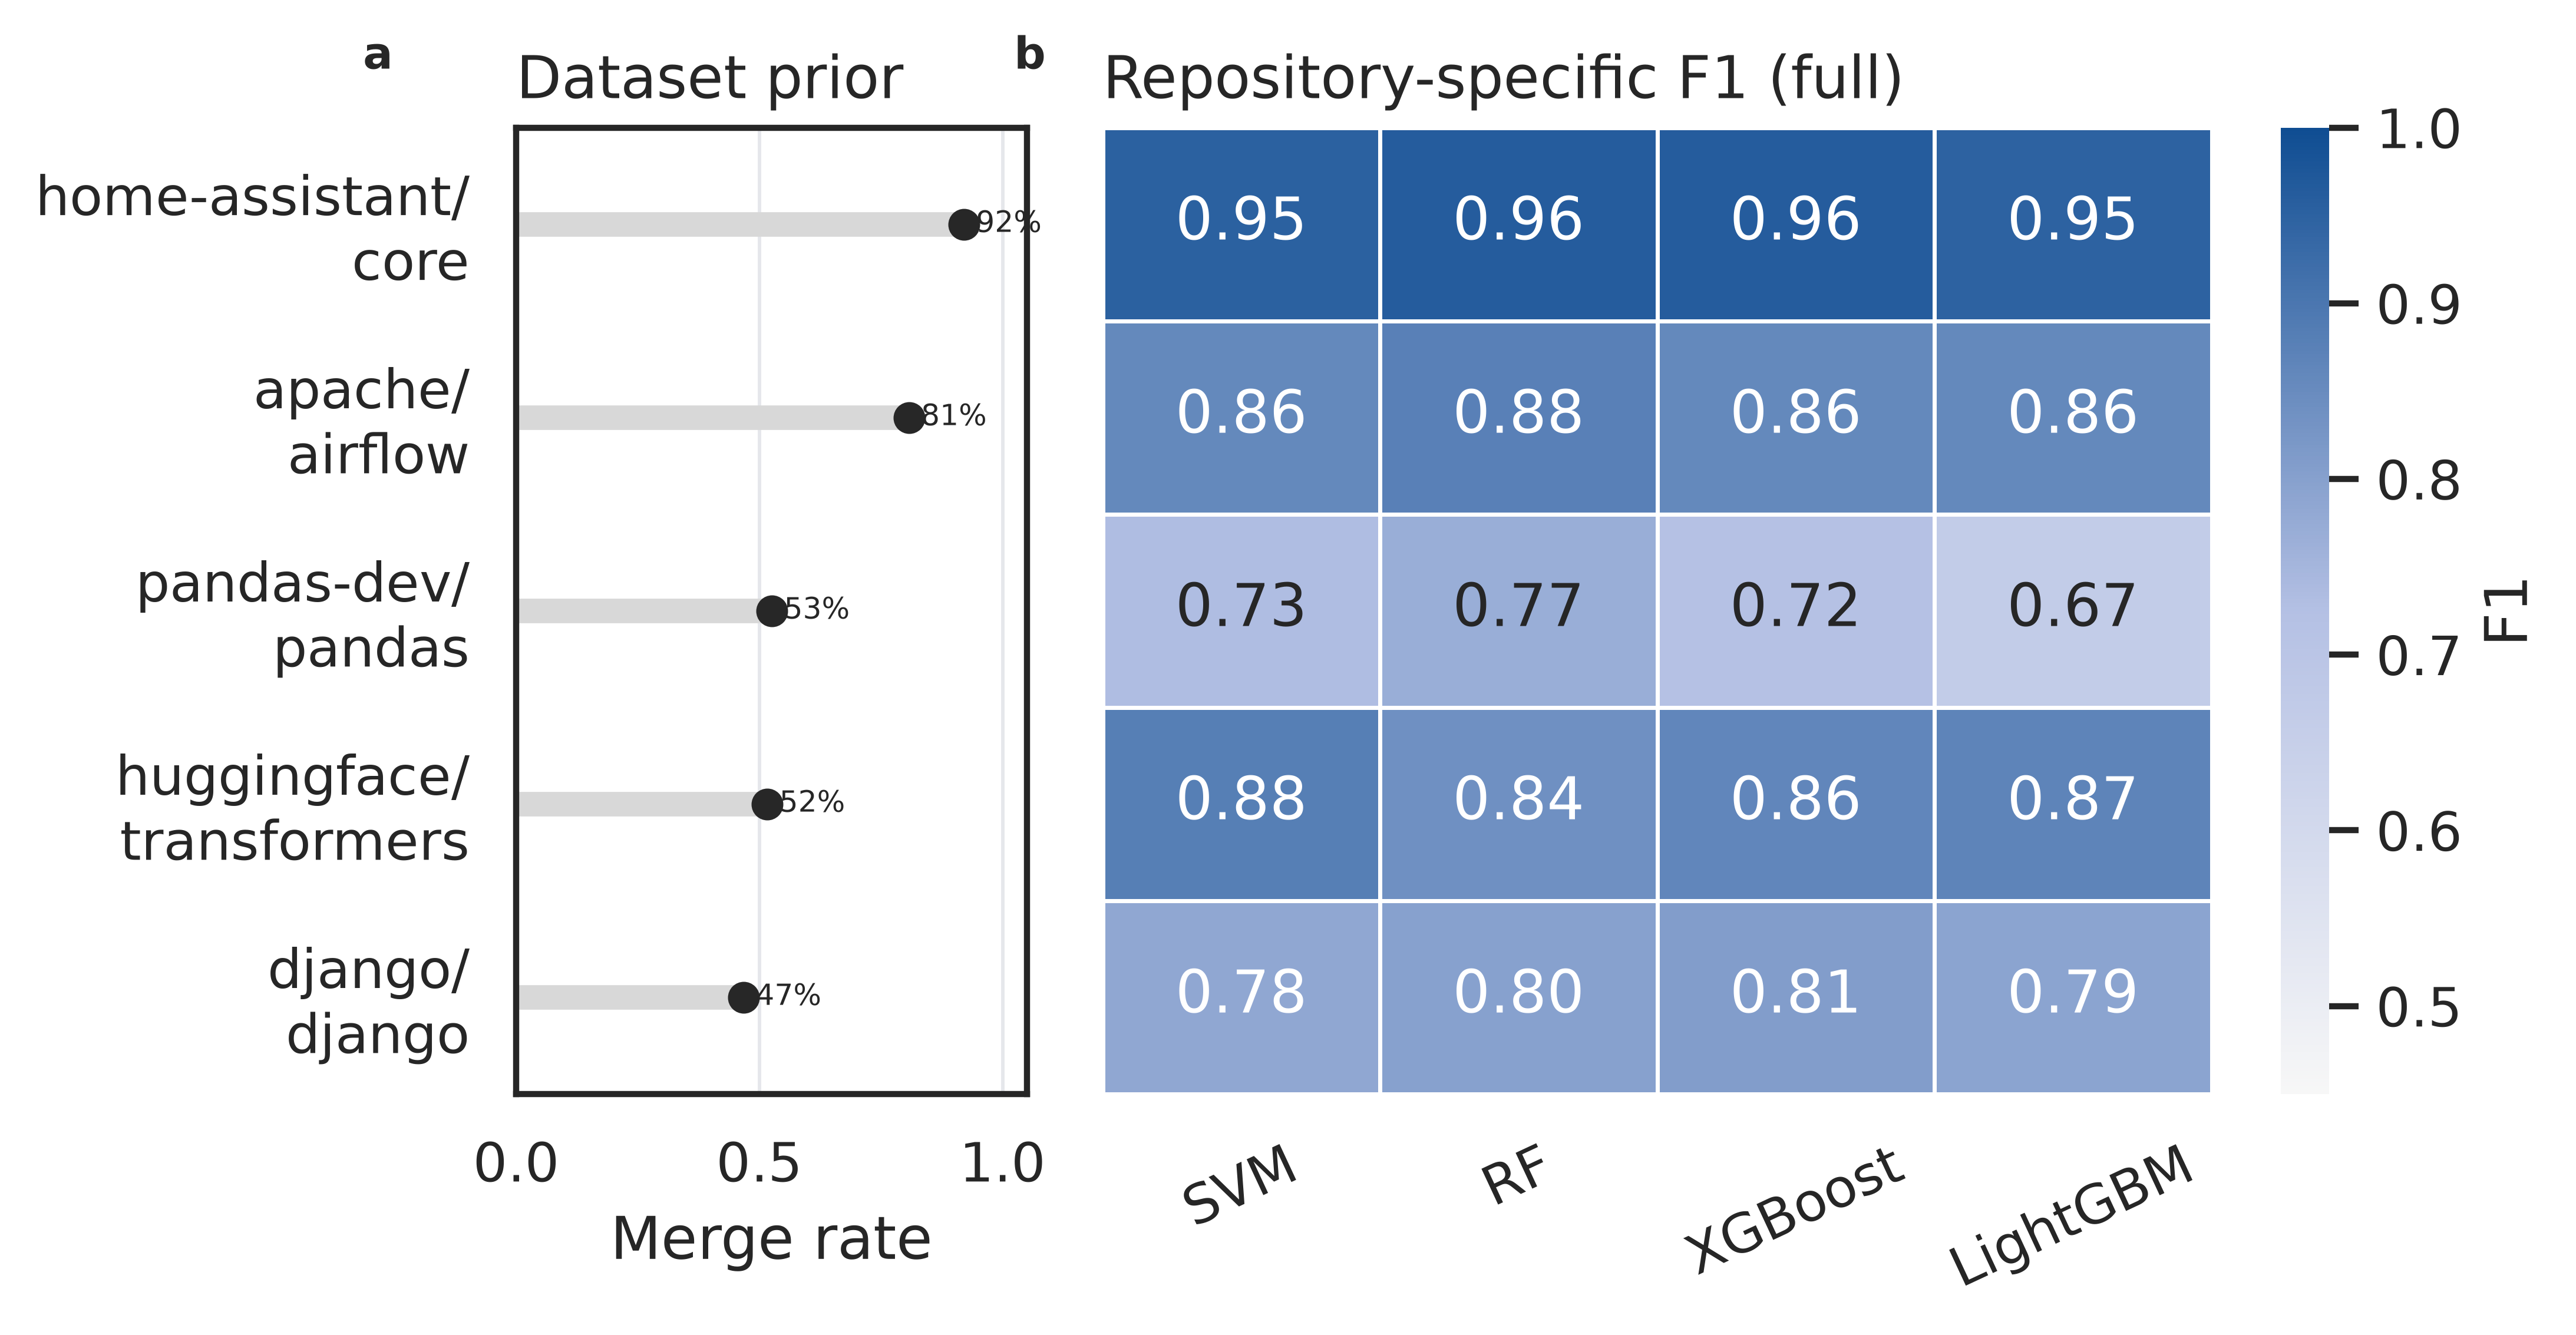
\includegraphics[width=\textwidth]{cross_repo_performance_full.png}
  \caption{Full 设置}
  \label{fig:repo-full}
\end{subfigure}
\caption{\textbf{分仓库 F1 性能。} 左侧条形为各仓库在建模数据集中的合并率，热力图给出测试集上各模型的分仓库 F1。(a) pre-review 下高合并率仓库易预测、类别均衡仓库（如 \texttt{django/django}）明显更难；(b) full 下审查过程特征对此前困难的仓库提升最大。}
\label{fig:repo}
\end{figure}

\subsection*{3.6 训练效率}

最后记录各模型训练时间以印证基线的成本定位（图~\ref{fig:time}）。在本次运行中，LightGBM 最快（0.021 s），SVM、XGBoost、RF 分别为 0.046 s、0.095 s、0.116 s；即便考虑运行环境波动，四类模型均属亚秒级的轻量训练流程。结合 3.4 节的特征重要性分析可知，传统 ML 的定位由此清晰：它未必能充分学习代码语义，但能以极低成本提供\textbf{可解释、可快速复现}的性能参照，非常适合作为后续 CodeBERT、LLM 与 VSCode 插件实验的基线。

\begin{figure}[H]
\centering
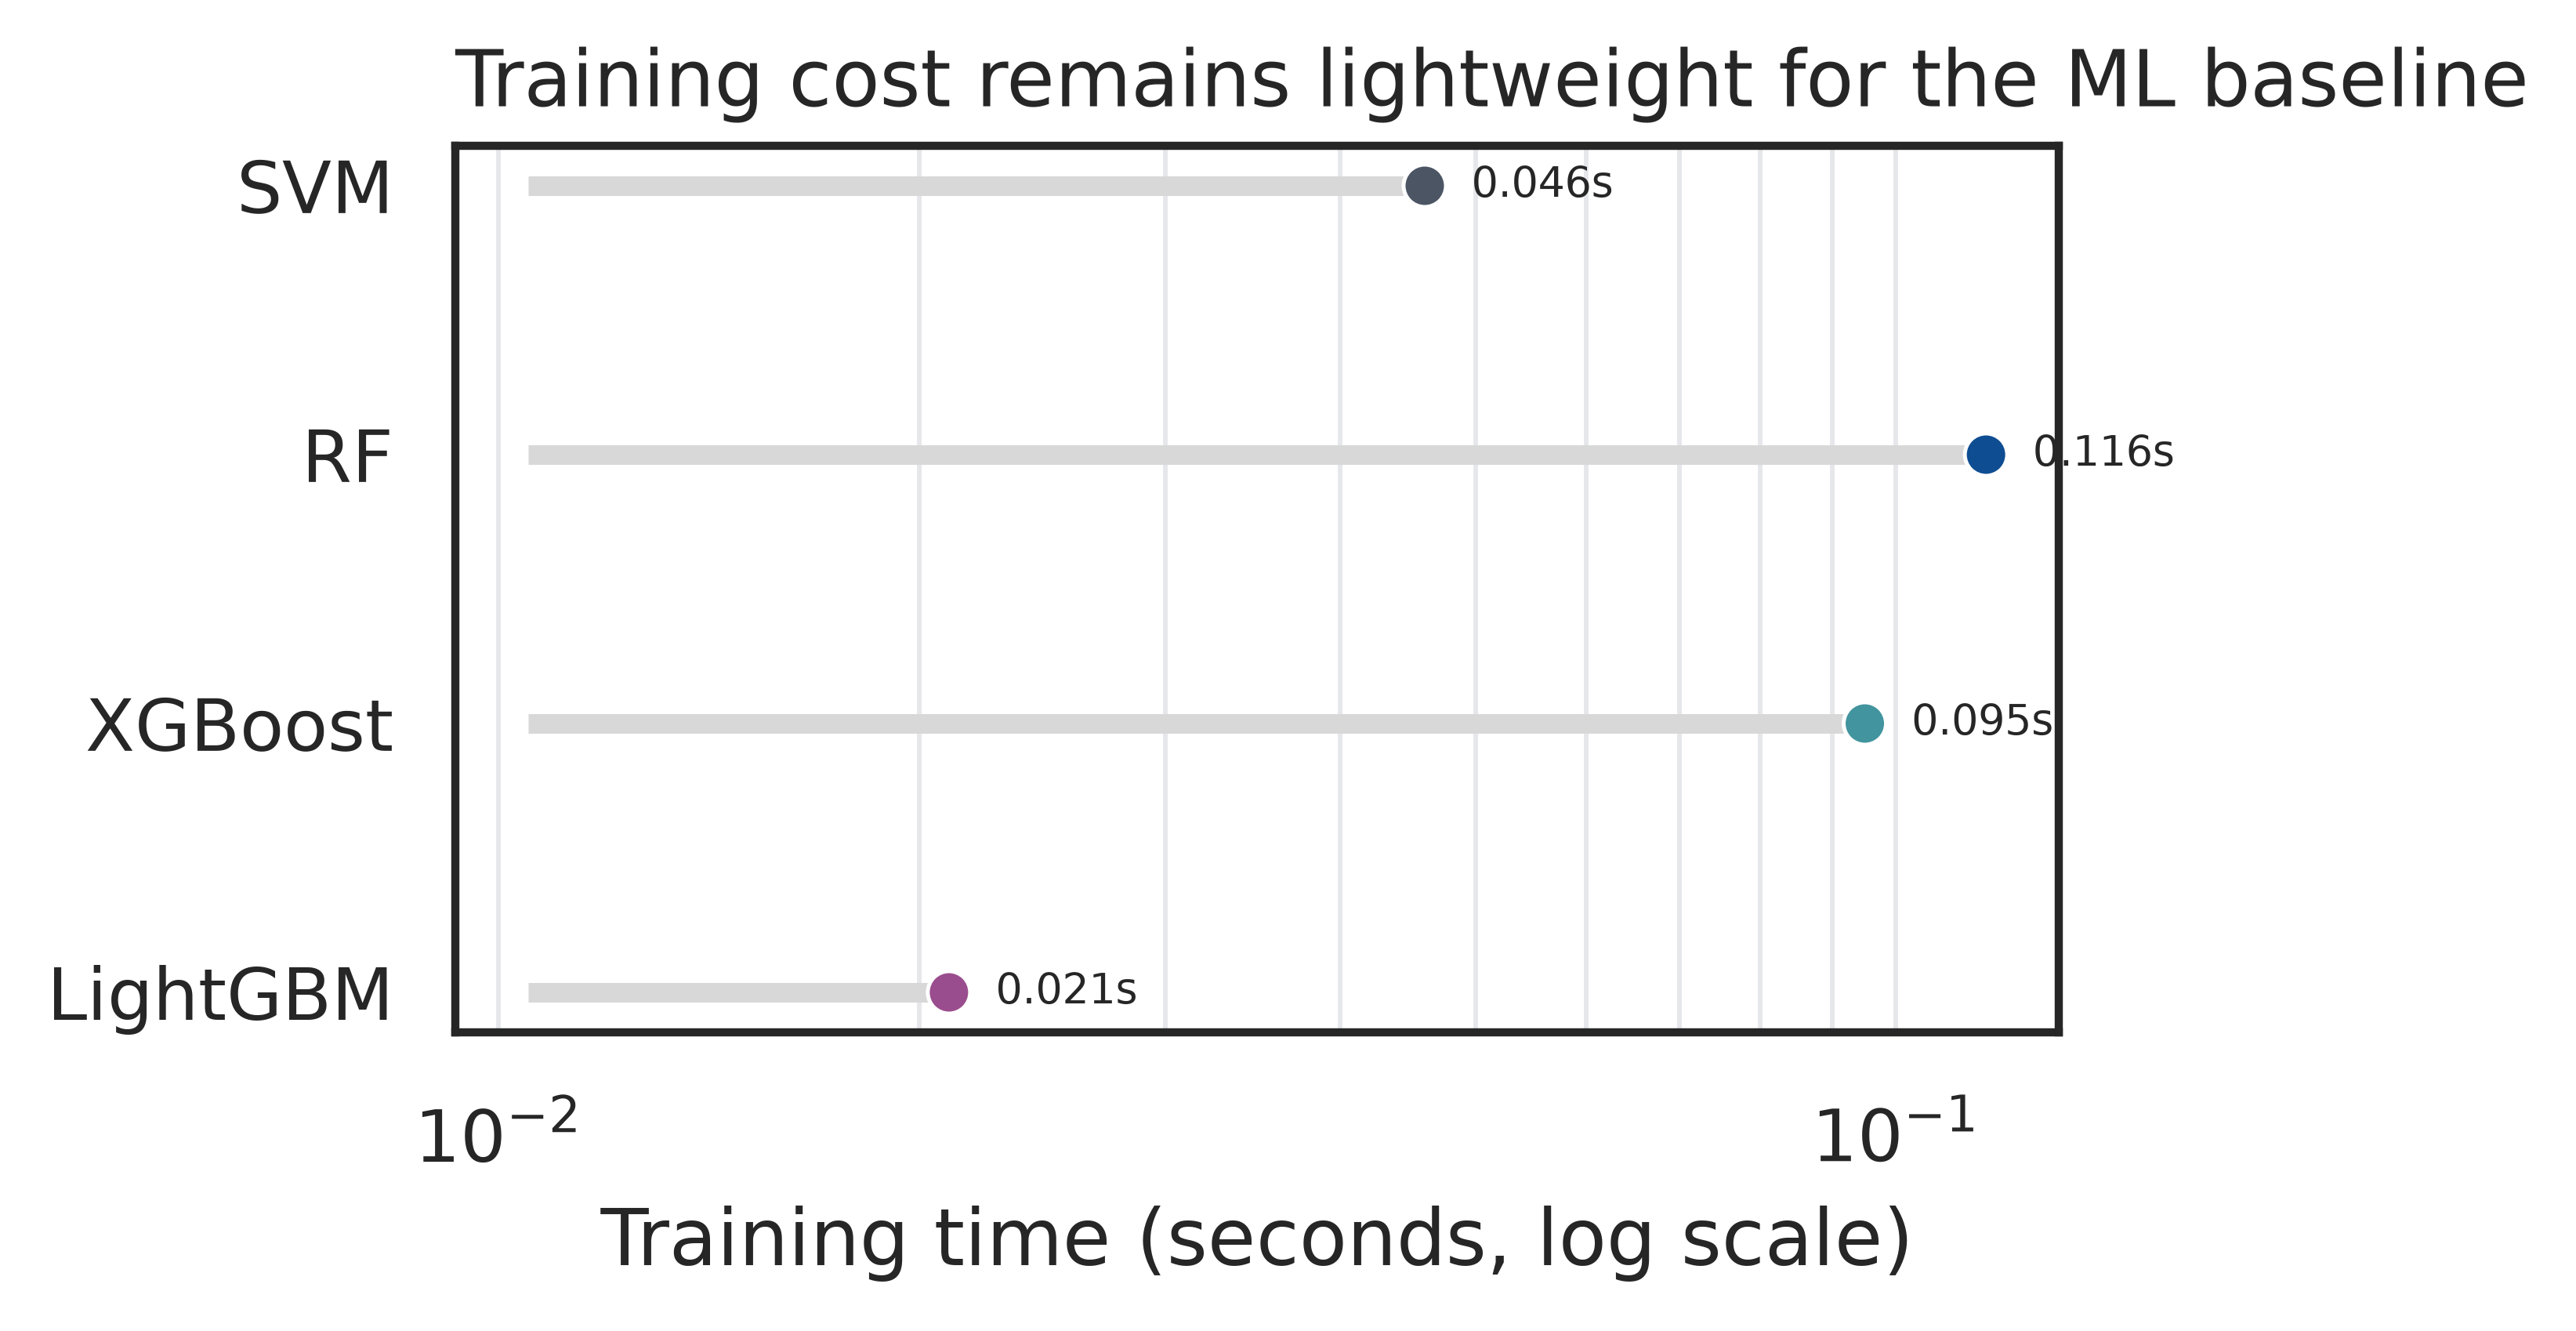
\includegraphics[width=0.7\textwidth]{training_time.png}
\caption{\textbf{传统机器学习基线的训练时间。} 点图采用对数横轴，因本次运行中所有模型均在亚秒内完成训练。四类模型均属轻量流程，适合作为下游深度学习与大语言模型方法的可复现基线。}
\label{fig:time}
\end{figure}

\subsection*{3.7 结果小结}

综合上述分析，本实验建立了一个可复现、低成本且可解释的传统机器学习 Merge Prediction 基线。在真实可部署的 pre-review 设置下，RF 取得最优 F1（0.813）与 ROC-AUC（0.834），表明人工特征已能提供稳定的合并预测信号，其中文本上下文与改动规模贡献最大、AST 结构次之、CFG 较弱；full 设置将 RF 的 F1、ROC-AUC 分别提升至 0.870 与 0.913，但特征重要性分析显示该提升主要由 \texttt{num\_reviews}、\texttt{num\_reviewers} 等审查过程特征驱动，故应解释为含时间泄漏的理论上界。跨仓库分析进一步表明 Merge Prediction 存在显著的仓库级分布偏移。这些结论共同为后续实验界定了可部署基线、上界参照与改进方向。

}

%========================
% 问题总结
%========================

\experimentproblems{

\subsection*{4.1 diff-only 条件下的代码结构特征提取}

本实验遇到的第一个问题是实验一保存的是 PR diff，而不是完整仓库文件。若直接把 patch 当作完整 Python 文件解析，修改类文件往往只包含局部 hunk，AST 中会出现残缺结构；若重新拉取仓库文件，又会引入网络依赖和 GitHub API 成本，也会越过实验六才需要处理的 repository 级上下文边界。对此，我们采用 diff-only 方案：从 patch 中保留上下文行和新增行、丢弃删除行，重建“改动后代码片段”，再使用 tree-sitter-python 进行容错解析。对于 CFG，则不追求完整语义级控制流图，而是用控制流语句、判定点和嵌套深度构造轻量统计特征。这样既保持了实验的自包含和可复现，也满足本实验对 AST/CFG 聚合统计特征的要求。

\subsection*{4.2 审查过程特征带来的标签泄漏}

第二个问题是部分特征虽然预测能力很强，但在真实部署时不可提前获得。例如 \texttt{num\_reviews}、\texttt{num\_reviewers} 和评论数量都发生在 PR 创建之后，若直接用于训练，会使模型学习到未来信息，从而高估 Merge Prediction 的实际能力。解决方法是显式区分两套特征集：pre-review 只使用 PR 提交时可得的 AST、CFG、改动统计和文本特征，作为可部署基线；full 在此基础上加入审查过程特征，只作为理论上界。后续结果分析也始终围绕这一区分展开，避免把含泄漏结果误解释为真实插件场景下的性能。

\subsection*{4.3 类别不平衡与跨仓库分布偏移}

第三个问题是数据并非完全均衡，不同仓库的合并率和审查风格也存在明显差异。若只做普通随机划分，可能导致某些仓库在训练集或测试集中代表性不足，整体指标也容易掩盖仓库级差异。对此，数据划分按仓库进行分层，训练、验证和测试集索引保持零重叠；模型训练时，SVM 与 RF 使用 \texttt{class\_weight=balanced}，XGBoost 和 LightGBM 分别使用对应的不平衡处理参数。同时，实验结果除总体指标外还报告分仓库 F1，以观察模型在不同项目上的泛化表现。

\subsection*{4.4 特征维度固定与结果可解释性}

第四个问题是 PR 的 diff、标题、正文和 commit message 都是变长信息，不能直接输入传统机器学习模型。为此，我们将代码结构信息聚合为 PR 级 AST/CFG 统计量，将改动规模归纳为数值特征，并对标题与正文使用 TF-IDF 提取固定维文本特征。训练时只在训练集上拟合标准化器，再应用到验证集和测试集，避免统计量泄漏。结果解释方面，主要读取 Random Forest 的特征重要性，从特征家族和单个特征两个层面分析模型依赖的信号，使实验不仅有预测指标，也能回答“哪些信息影响合并判断”这一问题。

}

%========================
% 实验体会
%========================

\experimentexperience{

\subsection*{5.1 对传统机器学习基线的认识}

通过本实验可以看到，传统机器学习虽然表达能力不如后续的 CodeBERT 或大语言模型，但在代码审查任务中仍然有明确价值。它训练速度快、实现成本低，并且能通过特征重要性解释模型决策。在 pre-review 设置下，RF 已能取得较稳定的 F1 和 ROC-AUC，说明人工设计的文本、改动规模和结构特征确实包含有效的合并预测信号。因此，传统 ML 更适合作为后续复杂模型的低成本、可解释基线，而不是简单地被视为过时方法。

\subsection*{5.2 对实验协议的认识}

本实验最重要的收获是：模型性能不能脱离数据协议解释。同样是 Merge Prediction，使用 pre-review 特征和使用 full 特征得到的结论并不相同。前者对应 PR 刚提交时的真实预测场景，后者包含审查过程信息，只能表示上界。如果不主动识别标签泄漏，模型指标会看起来更好，但结论反而不可靠。由此可见，在智能软件工程实验中，数据可获得时间、训练测试划分和评估场景往往和模型选择同样重要。

\subsection*{5.3 对后续实验的支撑}

实验二也进一步明确了后续实验的方向。首先，pre-review 结果可以作为实验三深度学习模型和实验四大语言模型的比较基线；其次，full 结果说明审查过程信息确实有价值，但需要在合适的任务阶段使用；最后，跨仓库分析表明不同项目之间存在分布偏移，后续若要做更强的模型或 VSCode 插件，应考虑仓库级上下文、项目审查习惯和更细粒度的 diff 语义。整体来看，本实验把实验一的数据基础转化为了可训练、可评估、可解释的 Merge Prediction 流水线，为后续实验提供了清晰参照。

}

%========================
% 教师评语
%========================

\teachercomment

\end{document}
